\documentclass[12pt]{report}
\ProvidesPackage{musereum}

\usepackage{graphicx}
\graphicspath{ {images/} }
\usepackage[T1]{fontenc}
\usepackage{titlesec, blindtext, color}
\definecolor{gray75}{gray}{0.75}
\newcommand{\hsp}{\hspace{20pt}}
\titleformat{\chapter}[hang]{\Huge\bfseries}{\thechapter\hsp\textcolor{gray75}{|}\hsp}{0pt}{\Huge\bfseries}
\titlespacing*{\chapter}{0pt}{-35pt}{40pt}

\usepackage{amsmath}
\usepackage{amsfonts}
\usepackage{amssymb}
\usepackage{booktabs}
\usepackage{pgfplots}
\usepackage{multirow}

\usepackage{tikz}
\usetikzlibrary{calc,trees,positioning,arrows,chains,fit,shapes.geometric,%
    decorations.pathreplacing,decorations.pathmorphing,shapes,%
    decorations.markings,%	
    matrix,shapes.symbols}


\usepackage{amsmath}
\usepackage{graphicx}
\usepackage{hyperref}
\hypersetup{
    colorlinks=true,
    linkcolor=blue,
    filecolor=magenta,      
    urlcolor=cyan,
}
%Russian-specific packages
%--------------------------------------
\usepackage[T2A]{fontenc}
\usepackage[utf8]{inputenc}
\usepackage[russian]{babel}
%--------------------------------------
 
%Hyphenation rules
%--------------------------------------
\usepackage{hyphenat}
\hyphenation{ма-те-ма-ти-ка вос-ста-нав-ли-вать}
%--------------------------------------

\usepackage{multicol}
\setlength{\columnsep}{1.2cm}

\newcommand{\hlc}[1]{\colorbox{yellow!25}{#1}}

\usepackage[a4paper, total={7in, 9.1in}]{geometry}

\tikzstyle{event} = [trapezium, trapezium left angle=70, trapezium right angle=110, minimum width=3cm, minimum height=1cm, text centered, draw=black]
\tikzstyle{inout} = [rectangle, rounded corners, minimum width=3cm, minimum height=1cm,text centered, draw=black]
\tikzstyle{rect} = [rectangle, minimum width=3cm, minimum height=1cm, text centered, draw=black]
\tikzstyle{check} = [diamond, minimum width=3cm, minimum height=1cm, text centered, draw=black]
\tikzstyle{arrow} = [thick,->,>=stealth]
\tikzstyle{line} = [thick]
\tikzstyle{vecArrow} = [thick, decoration={markings,mark=at position
   1 with {\arrow[semithick]{open triangle 60}}},
   double distance=1.4pt, shorten >= 5.5pt,
   preaction = {decorate},
   postaction = {draw,line width=1.4pt, white,shorten >= 4.5pt}]
\tikzstyle{innerWhite} = [semithick, white,line width=1.4pt, shorten >= 4.5pt]

\pgfdeclarelayer{background}
\pgfdeclarelayer{foreground}
\pgfsetlayers{background,main,foreground}

%\usepackage{musereum}
\usepackage{import}

\setlength{\parindent}{0em}
\setlength{\parskip}{0.65em}
\renewcommand{\baselinestretch}{1.1}

\definecolor{light-gray}{gray}{0.95}
\def\code#1{\colorbox{light-gray}{\texttt{#1}}}

\title{Musereum}
\author{Artem Aler Dan}
\date{\today}

\begin{document}
\maketitle
\pagebreak
\tableofcontents
\pagebreak

\chapter{Введение}
\label{overview}
\begin{multicols}{2}
\hlc{«Musereum»} – это мульти-блокчейн проект, созданный консорциумом блокчейн-профессионалов в сотрудничестве с экспертами в разработке программного обеспечения, юристами и профессиональными участниками музыкальной индустрии, способными применить сильные стороны указанных сфер и технологии для решения реальных бизнес-задач, а также преобразования мировой музыкальной индустрии в целом.

Проект представляет собой музыкальную платформу, сформированную на базе смарт-контрактов. Токены «Musereum» являются основополагающей единицей на платформе для построения экономических взаимоотношений между всеми участниками сети.

Мы понимаем, что изменить текущую ситуацию в индустрии, которая формировалась десятки лет, в один момент не получится, поэтому инновационные механизмы будут внедряться постепенно в коллаборации c заинтересованными сторонами процесса. 

В рамках проекта «Musereum» участники смогут создавать токены, в которые будет “упакована” доля в совместном исключительном праве на музыкальное произведение. Эмиссия таких токенов будет сопровождаться лицензированием того или иного объекта музыкального произведения и таймштампингом в публичной сети Ethereum или Ethereum Classic. Музыкальные токены будут свободно обмениваться на авторизованных биржах, позволяя музыкантам привлекать средства по модели краудинвестинга, профессиональным участникам рынка – использовать прозрачный инструмент для очистки прав на музыкальные произведения, слушателям – иметь легальную возможность напрямую поддерживать любимого автора, а инвесторам – получить новый инвестиционный инструмент.

Результатом реализации проекта станет коренное изменение отношений, складывающихся в музыкальной сфере, а именно:

\begin{itemize}
	\item создание базы данных для управления правами интеллектуальной собственности;
	\item достижение справедливости при выплате роялти посредством децентрализации процессов;
	\item создание музыкальной платформы для начинающих талантов;
	\item упрощение процедуры лицензирования.
\end{itemize}
\end{multicols}

\chapter{Обзор индустрии}
\label{industry}
%\begin{multicols}{2}
Уже к середине 2017 года общее потребление музыки выросло на 9,9\% по сравнению с прошлым годом. 

Аналитическая компания «Buzzanngelmusic» провела исследование музыкального рынка и пришла к следующим выводам: общий объем потребления музыкальных альбомов вырос на 9\%, а музыкальных произведений - на 29,5\%.  
%\end{multicols}

\def\Prev{2016 год}
\def\Current{2017 год}
\def\Grow{\% роста}
\def\Summary{Общее потребление музыкальных произведений}
\def\Sales{Продажи песен}
\def\Streaming{Потоковое вещание}
\def\VideoStreaming{Видео вещание}
\def\Albums{Общее потребление альбомов}
\def\AlbumsSales{Продажи альбомов}
\def\TracksSales{Продажи песен}

\begin{table}[h]
\centering
\caption{Предзаготовленные типовые ограничения лицензий}
\begin{tabular}{p{0.45\linewidth}rrr}%p{0.65\linewidth}cc}
\toprule
& \Prev & \Current & \Grow \\
\bottomrule
\toprule
%\multicolumn{2}{c}{\code{EnumerateRule}} \\
\midrule
\Summary 			& 1,167,384,931 		& 1,512,049,118 		& 29.5\% \\
\Sales 					& 410,920,611 			& 313,305,154 			& -23.8\% \\
\Streaming 			& 113,469,648,006 	& 179,811,594,535 	& 58.5\% \\
\VideoStreaming 	& 95,696,158,924 	& 101,531,507,971		& 6.1\% \\
\Albums 				& 266,565,904 		& 292,986,056 		& 9.9\% \\
\AlbumsSales 		& 86,029,972 			& 74,093,472	 		& -13.9\% \\
\bottomrule
\end{tabular}
\end{table}

\vfill\null\pagebreak
\section{Artem}
\label{industry-distribution}

\newcommand{\slice}[4]{
  \pgfmathparse{0.5*#1+0.5*#2}
  \let\midangle\pgfmathresult

  % slice
  \draw[thick,fill=black!10] (0,0) -- (#1:1) arc (#1:#2:1) -- cycle;

  % outer label
  \node[label=\midangle:#4] at (\midangle:1) {};

  % inner label
  \pgfmathparse{min((#2-#1-10)/110*(-0.3),0)}
  \let\temp\pgfmathresult
  \pgfmathparse{max(\temp,-0.5) + 0.8}
  \let\innerpos\pgfmathresult
  \node at (\midangle:\innerpos) {#3};
}

\def\Royalty{Авторские права}
\def\Digital{Цифровые форматы}
\def\Physical{Физические носители}
\def\Sync{Синхронизация}

\begin{figure}[h]
\centering
\caption{Доходы от распространения музыкального произведения}
\begin{tikzpicture}[scale=3]

\newcounter{a}
\newcounter{b}
\foreach \p/\t in {
	14/\Royalty, 
	50/\Digital, 
	34/\Physical,
	2/\Sync}
  {
    \setcounter{a}{\value{b}}
    \addtocounter{b}{\p}
    \slice{\thea/100*360}
          {\theb/100*360}
          {\p\%}{\t}
  }

\end{tikzpicture}
\end{figure}

Такая популярность обусловлена соответствующим ростом доходности. Стоит отметить, что наибольший доход приносят произведения, распространяемые на цифровых форматах, которые составляют ровно половину всей потребляемой музыки, в отличии от тех, например, которые распространяются посредством  физических продаж - 34\%, согласно данным 

\begin{figure}[h]
\centering
\caption{Доходы от потокового вещания}
\vspace{20pt}
\pgfplotstableread[row sep=\\,col sep=&]{
    interval & carT \\
    2011 	& 10 \\
    2012 & 15 \\
    2013 & 21 \\
    2014 & 25 \\
    2015 & 32 \\
    2016 & 50 \\
    }\streamingPartion
\begin{tikzpicture}
    \begin{axis}[
            ybar,
            symbolic x coords={2011,2012,2013,2014,2015,2016},
            xtick=data,
            nodes near coords,
            ymin=0,ymax=65,
            width=13cm, %set bigger width
		   height=6cm,
		   bar width=1.5cm,
            ylabel={Доля дохода, \%},
        ]
        \addplot table[x=interval,y=carT]{\streamingPartion};
    \end{axis}
\end{tikzpicture}
\end{figure}

В 2017 году аудиостриминг достиг рекордных отметок и вырос на 58,5\%. На отдельных рынках рост доходности достигал более 300\% (Южная Африка).
По доходности аудиостриминг является лидером в своей сфере. К примеру, несмотря на то, что видео направление привлекает 900 млн пользователей, прибыль составила всего \$553 млн, в то время как, доход от потокового вещания равен 3,904 млн, а общее количество пользователей 212 млн.

\begin{figure}[h]
\centering
\caption{Аудио- и видео-стриминг: соотношение количества пользователей и прибыли}
\vspace{20pt}
\pgfplotstableread[row sep=\\,col sep=&]{
    interval & users & revenue \\
    1 & 250 & 3950 \\
    2 & 920 & 550 \\
    }\userRevenue
\begin{tikzpicture}
    \begin{axis}[
            ybar,
            symbolic x coords={1,2},
            xtick=data,
            nodes near coords,
            ymin=0,ymax=4500,
            ylabel={Доля дохода, \%},
        ]
        \addplot table[x=interval,y=users]{\userRevenue};
        \addplot table[x=interval,y=revenue]{\userRevenue};
    \end{axis}
\end{tikzpicture}
\end{figure}	

Несомненно, затраты на раскрутку одной композиции требует средств.
В среднем инвестиции в новую запись составляют US\$498 000 - 2 000 000 (в частности, именно такие цифры подтверждают данные из США и Великобритании). В 2015 году  было инвестировано US\$4.5 млрд в A\&R и Marketing прибыли всей мировой музыкальной индустрии.

\def\InvestToRecord{Инвестиции в раскрутку новой записи}
\def\Clients{Привлечение клиентов}
\def\Record{Затраты на запись}
\def\Video{Видео}
\def\Tour{Поддержка тура}
\def\Marketing{Маркетинг}
\def\Sum{Итого}

\begin{table}[h]
\centering
\caption{Инвестиции в раскрутку новой записи}
\begin{tabular}{p{0.5\linewidth}r}
\toprule
\multicolumn{2}{c}{\InvestToRecord} \\
\bottomrule
\midrule
\Clients					& US \$50.000-350.000 \\
\Record					& US \$150.000-500.000 \\
\Video					& US \$25.000-300.000 \\
\Tour					& US \$50.000-150.000 \\
\Marketing			& US \$200.000-700.000 \\
\Sum 					& US \$475.000-2.000.000 \\
\bottomrule
\end{tabular}
\end{table}

На популярность музыкального произведения влияет и популярность артиста, его исполняющего, что, в наше время, напрямую связано с использованием социальных сетей. 6 из 10 наиболее понравившихся людей на Facebook, followed на Twitter, просматриваемых видео на Youtube – музыкальные исполнители.

Также необходимо учитывать международный характер потокового вещания. 230 цифровых музыкальных сервисов предлагают доступ к 40 млн треков на территории всего ЕС. При этом, около 50\% всех популярных треков, загруженных и проигрываемых в Европе, не европейского производства.  

Наибольший процент прибыли в 2016 года, а именно, 50\%, мировому рынку музыкальной индустрии принесли именно музыкальные произведения в цифровом формате, общая сумма составила US\$15.7 млрд.

IFPI утверждает, что 50\% доходов от записи поступают субъектам музыкальной индустрии именно благодаря наличию цифровых форматов. 

К примеру, цифровые платформы выплачивают следующий процент:


\def\PayPlay{Оплата за прослушивание}
\def\PayBuy{Оплата при покупке песни}
\def\Platform{Музыкальная платформа}
\def\LabelPartion{Отчисления для лейбла}
\def\ArtistPartion{\% отчислений, попадающих артисту}
\def\YoutubePay{отчисление осуществляется в размере \$0,001 субъекту, разместившему произведение}

\begin{table}[h]
\centering
\caption{Выплаты платформ}
\begin{tabular}{lrrp{0.15\linewidth}}
\toprule
	& \multicolumn{2}{c}{\PayPlay} \\
	\Platform & 
	\multicolumn{1}{p{0.22\linewidth}}{\LabelPartion} &
	\multicolumn{1}{p{0.22\linewidth}}{\ArtistPartion} \\
\bottomrule
\midrule
Apple Music / iTunes		& US \$0.0013 	& 12\% \\
Zune								& US \$0.028 	& 11\% \\
Napster						& US \$0.016 	& 11-12\% \\
Rhapsody						& US \$0.013 	& 11-12\% \\
Spotify							& US \$0.005 	& 11-12\% \\
Youtube 						& \multicolumn{2}{p{0.48\linewidth}}{\YoutubePay} \\
\bottomrule
\end{tabular}
\end{table}

Но платформа и артист являются не единственными субъектами музыкальной индустрии.

Поскольку схема правоотношений оказывается крайне громоздкой, конечному пользователю, желающему получить лицензию на использование музыкального произведения, зачастую приходится обращаться к еще одному профессиональному игроку на рынке – к агентству по очистке прав, которое либо урегулирует отношения между всеми правообладателями, либо просто выкупает права на музыкальное произведение.

Таким образом, основными игроками музыкальной индустрии являются:

\vfill\null\pagebreak
\section{Структура музыкальной индустрии}
\label{industry-structure}
\begin{multicols}{2}
Кажется очевидным, что центральной концепцией и итоговым продуктом, которым обусловлено само существование музыкальной индустрии, является музыка. Однако само это понятие является неоднородным, и именно благодаря этому вместо прямых отношений «Музыкант – слушатель», существовавших в каменном веке, мы имеем сложную, запутанную и не всегда эффективно работающую структуру.

Стоит сказать, что музыка совмещает в себе два объекта:
\begin{enumerate}
	\item музыкальное произведение (инструкция по исполнению музыки), 
	\item фонограмма (исполненная и сохраненная на материальном носителе музыка).
\end{enumerate}

В отношении каждого из этих объектов действует исключительное право, то есть, право определять порядок использования и получать вознаграждение за такое использование. Исключительным правом на музыкальное произведение обладают его авторы (композитор, автор текста), на фонограмму - исполнитель и изготовитель фонограммы. В самой простой ситуации, автор, исполнитель и изготовитель фонограммы оказываются одним человеком – однако, это редкость.

Таким образом, для использования музыки по общему правилу требуется получить разрешение авторов, исполнителей и изготовителей фонограммы,но музыканты редко самостоятельно управляют своими правами. 

Исполнитель обычно обращается к звукозаписывающей компании – лейблу – и получает от него аванс в обмен на право лейбла удерживать часть роялти от дальнейшего использования музыки; зачастую при этом лейблу передаются и исключительные права на исполнение. 

Лейблы можно разделить на два основных вида: мэйджоры (the majors) и инди-лейблы (the independents). Первые являются крупными звукозаписывающими компаниями, вторые представляют микро-, малый и средний бизнес индустрии. Несмотря на это, именно на долю последних приходится 80\% всех новых релизов,  самый крупный из них занимает всего лишь 1,5\% рынка. На мировом рынке индустрии инди-лейблы составляют 37,6\% и оцениваются в \$5.6 млрд. В среднем они работают с 40 артистами. Обоим видам лейблов потоковое вещание приносит  наибольшую долю прибыли. 

Право изготовителя фонограммы также обычно принадлежит лейблу, хотя может удерживаться и исполнителем. Авторы, в свою очередь, передают свои права в управление музыкальному издательству – паблишеру – занимающемуся защитой авторских прав в обмен на часть дохода от использования произведения. 

Распространением и доведением музыки до конечного пользователя занимаются дистрибьюторы (распространяющие музыку на физических носителях) и агрегаторы (распространяющие музыку в цифровом формате).

Поскольку даже крупные правообладатели не в состоянии отслеживать любое использование принадлежащей им музыки, в большинстве государств создаются организации по коллективному управлению правами (ОКУП). ОКУПы отслеживают случаи публичного использования произведений и взимают плату за такое использование, которая потом тем или иным способом распределяется между правообладателями; при этом обычно для каждого типа исключительных прав действует отдельный ОКУП. В некоторых странах такие организации существуют только для определенных типов прав. Кроме этого, в отдельных странах (Россия, скандинавские государства) ОКУПы управляют правами на бездоговорной основе – то есть имеют права взыскивать роялти в пользу правообладателей, не имеющих с ОКУПом никаких отношений.

Таким образом, примерная структура создания ценности в музыкальной индустрии выглядит следующим образом:

\end{multicols}

\begin{figure}[h]
\centering

\def\Author{Автор}
\def\AuthorDesc{Создает оригинальные музыкальные произведения; может передавать права на публикацию за долю роялти составляющую не более 50\%}
\def\Publisher{Издательство}
\def\PublisherDesc{Лицензирует каталог музыкальных произведений для воспроизведения и механического использования; собирает и распределяет роялти между авторами}
\def\Laws{Правовое общество}
\def\LawsDesc{Отслеживает и оценивает каждое использование композиций; собирает и распределяет роялти между авторами и издательствами}
\def\LawNote{Право на музыкальное произведение принадлежит автору или издательству; Использование в рамках воспроизведения отслеживается правовым обществом}
\def\LicensePlay{Лицензия на воспроизведение}
\def\LicensePhysical{Механическая лицензия}

\def\Artist{Записывающий исполнитель}
\def\ArtistDesc{Основные и бэк-исполнители, участвующие в звукозаписи в обмен на роялти с продаж}
\def\Label{Лейбл}
\def\LabelDesc{Спонсирует, записывает и продвигает аудиозаписи}
\def\Distributor{Агрегатор / Дистрибьютер}
\def\DistributorDesc{Распространяет цифровые аудиозаписи онлайн или физические продукты через магазин}
\def\LawSecondNote{Право на аудиозапись принадлежит автору или лейблу; продажи отслеживают лейблом, агрегатором или дистрибьютером}
\def\Records{Аудиозаписи}
\def\Around{Смежные права}

\caption{Структура создания ценности}
\vspace{20pt}
\begin{tikzpicture}[node distance=1.5cm]
\node(Author) 			[rect, text width=5.1cm]
								{\textbf{\Author}\linebreak\AuthorDesc};
\node(Publisher)		[rect, text width=5.1cm, below=0.5cm of Author]
								{\textbf{\Publisher}\linebreak\PublisherDesc};
\node(Laws)				[rect, text width=5.1cm, below=0.5cm of Publisher]
								{\textbf{\Laws}\linebreak\LawsDesc};

\node(LawNote)		[inout, text width=5.5cm, below=0.5cm of Laws]
								{\LawNote};
								
\node(LicensePlay)	[rect, text width=3.1cm, below=0.5cm of LawNote, anchor=north east, xshift=-.25cm]
								{\LicensePlay};
								
\node(LicensePhysical) [rect, text width=3.1cm, below=0.5cm of LawNote, anchor=north west, xshift=.25cm]
								{\LicensePhysical};
								

\node(Artist) 			[rect, text width=5.1cm, right=3cm of Author.north east, anchor=north west]
								{\textbf{\Artist}\linebreak\ArtistDesc};
\node(Label)				[rect, text width=5.1cm, below=0.5cm of Artist]
								{\textbf{\Label}\linebreak\LabelDesc};
\node(Distributor)		[rect, text width=5.1cm, below=0.5cm of Label]
								{\textbf{\Distributor}\linebreak\DistributorDesc};

\node(LawSecondNote)	[inout, text width=5.5cm, below=0.5cm of Distributor]
								{\LawSecondNote};
								
\node(Records)			[rect, text width=3.1cm, below=0.5cm of LawSecondNote.south, anchor=north east, xshift=-.25cm]
								{\Records};
								
\node(Around) 			[rect, text width=3.1cm, below=0.5cm of LawSecondNote.south, anchor=north west, xshift=.25cm]
								{\Around};
%\node (LoadByteCode)		[rect, text width=11.5em] 
%										{\LoadByteCode};

%\node (LoadSourceCode)	[rect, text width=11.5em, below of=LoadByteCode] 
%										{\LoadSourceCode};

%\node (ValidationEnded)	[event, text width=11.5em, below=1.5cm of LoadSourceCode]
%										{\ValidationEnded};
										
%\node (aux0)[right=2cm of ValidationEnded]{};
%\node (Invalid)					[text width=5em, above of=aux0]
%										{$\pi_{ended} = 0$};

%\node (ChangeStatus)		[rect, text width=11.5em, below of=ValidationEnded]	
%										{\ChangeStatus};

%\node (InDevelopment)		[inout, text width=11em, right=1cm of LoadByteCode]			
%										{$\rho_{stateOf}(a) = P_{development}$};
										
%\node (InProduction)			[inout, text width=11em, right=1cm of ChangeStatus]			
%										{$\rho_{stateOf}(a) = P_{development}$};

%arrows
%\draw [arrow] (LoadByteCode)				-- (LoadSourceCode);
%\draw [arrow] (LoadByteCode)				-- (InDevelopment);
%\draw [arrow] (LoadSourceCode) 			-- (ValidationEnded);
%\draw [arrow] (ValidationEnded)			-- (ChangeStatus);
%\draw [arrow] (ValidationEnded)			-| (Invalid);
%\draw [thick]  (Invalid)  							-| (ValidationEnded);
%\draw [arrow] (ChangeStatus)				-- (InProduction);

\end{tikzpicture} 
\end{figure}

\begin{figure}[h]
\centering
\caption{Аудио- и видео-стриминг: соотношение количества пользователей и прибыли}
\vspace{20pt}
\pgfplotstableread[row sep=\\,col sep=&]{
    interval & users & revenue \\
    1 & 250 & 3950 \\
    2 & 920 & 550 \\
    }\userRevenue
\begin{tikzpicture}
    \begin{axis}[
            ybar,
            symbolic x coords={1,2},
            xtick=data,
            nodes near coords,
            ymin=0,ymax=4500,
            ylabel={Доля дохода, \%},
        ]
        \addplot table[x=interval,y=users]{\userRevenue};
        \addplot table[x=interval,y=revenue]{\userRevenue};
    \end{axis}
\end{tikzpicture}
\end{figure}	

\begin{multicols}{2}
Поскольку схема правоотношений оказывается крайне громоздкой, конечному пользователю, желающему получить лицензию на использование музыкального произведения, зачастую приходится обращаться к еще одному профессиональному игроку на рынке – к агентству по очистке прав, которое либо урегулирует отношения между всеми правообладателями, либо просто выкупает права на музыкальное произведение.

\begin{itemize}
	\item Композиторы;
	\item Авторы текстов;
	\item Музыканты-исполнители;
	\item Лейблы;
	\item Паблишеры;
	\item Агентства по очистке прав;
	\item Дистрибьюторы и агрегаторы;
	\item Организации по коллективному управлению правами.
\end{itemize}
	
Каждое использование музыки создает поток роялти, распределяющиеся между всеми указанными игроками:
\end{multicols}

\begin{figure}[h]
\centering
\caption{Аудио- и видео-стриминг: соотношение количества пользователей и прибыли}
\vspace{20pt}
\pgfplotstableread[row sep=\\,col sep=&]{
    interval & users & revenue \\
    1 & 250 & 3950 \\
    2 & 920 & 550 \\
    }\userRevenue
\begin{tikzpicture}
    \begin{axis}[
            ybar,
            symbolic x coords={1,2},
            xtick=data,
            nodes near coords,
            ymin=0,ymax=4500,
            ylabel={Доля дохода, \%},
        ]
        \addplot table[x=interval,y=users]{\userRevenue};
        \addplot table[x=interval,y=revenue]{\userRevenue};
    \end{axis}
\end{tikzpicture}
\end{figure}	

\begin{multicols}{2}
Однако при этом реальные отношения в отношении музыки оказываются еще сложнее. 
	При создании современной музыки широко используется семплирование; при этом в информационно перенасыщенном пространстве невозможным становится создание абсолютно оригинального произведения, не содержащего заимствования. За каждым использованием в произведении семплом стоит такая же сложная структура прав, что делает получение лицензии на музыку фрактально сложным предприятием.

Эта сложность иллюстрируется заявлением RIAA, один из членов которой для выпуска альбома был вынужден получить 1481 лицензию от 51 автора с 89 долями, одна из которых представляла собой всего 1,5 процента от общего объема прав, но была разделена между двумя паблишерами.

Учитывая международный характер цифрового распространения музыки, о котором упоминалось выше, процесс еще больше усложняется, так как возникает необходимость учета особенностей правового регулирования отдельных юрисдикций. Так, в США, правообладатели не имеют права на получение вознаграждения при вещании их музыки по радио.
\end{multicols}
\vfill\null\pagebreak

\section{Основные проблемы музыкальной индустрии}
\label{industry-problems}
\begin{multicols}{2}
Чрезмерная усложненность структуры отношений в музыкальной индустрии ведет к возникновению общепризнанных проблем, которые в той или иной степени затрагивают всех участников отношений.

\subsection{Отсутствие доступной и достоверной информации о принадлежности прав}

Как указывает RIAA, «сложно идентифицировать и отслеживать принадлежность права на музыкальное произведение в связи с изменениями при переходе произведений и каталогов из рук в руки». Помимо необходимости отслеживания истории смены правообладателей, ситуация осложняется многослойностью музыки как объекта интеллектуальных прав – существованием отдельных прав на музыкальное произведение и аудиозапись, а также традиционной для нынешнего состояния индустрии множественностью правообладателей для каждого из таких слоев. Кроме этого, проблема заключается в отсутствии универсально принятых в индустрии идентификаторов данных. 

Эта ситуация ведет к отсутствию определенности для потенциальных лицензиатов – им неясно, с кем именно надо договариваться, чтобы получить возможность использовать музыку на законных основаниях. Музыкальный рынок частично решает эту проблема появлением нового типа игроков – агентств по очистке прав – однако это решение является субоптимальным, поскольку увеличивает количество работы, вынуждая специалистов затрачивать существенные ресурсы на работу со сложно отслеживаемой историей транзакций, вместо того, чтобы отслеживать и записывать эту историю в реальном времени. Результатом является существенное повышение стоимости музыкального произведения для конечного пользователя, который вынужден из своего кармана оплачивать борьбу с такой неопределенностью. 

Более того, некоторые композиторы и музыканты в связи с особо сложно отслеживаемой историей могут вообще оказаться лишены права на доведение своих произведений до конечного пользователя, как в силу отказа со стороны агентства по очистке прав, так и в результате дедлока между множественными правообладателями.

В настоящее время нет единой базы данных для хранения информации об авторских правах на музыкальное произведение. В книге “Биткойн для рок-звезд” Д.А. Уоллак объясняет это так: “Корень проблемы — отсутствие одного набора данных со сведениями об авторах и правах. Сегодня эта информация распылена между многими организациями, каждая из которых считает ее своей собственностью. Это вполне понятно, если учесть, что они инвестируют в свои наборы данных серьезные деньги”.

В 2011 году была предпринята попытка создать такую базу данных. При поддержке музыкальных издателей был запущен проект по составлению “Глобальной БД репертуара” (GRD). Предполагалось, что она станет центром регистрации всех звукозаписей и связанных с ними метаданных. Увы, в июле 2014 года проект был закрыт из-за претензий со стороны обществ по сбору авторских отчислений. 

\subsection{Непрозрачность транзакций в индустрии}

С первой проблемой неразрывно связана вторая. Даже если на определенный момент времени принадлежность прав на произведение или аудиозапись оказывается достоверно зафиксированным, отсутствуют универсальные решения, позволяющие убедиться в актуальности такой информации. Более того, в случае возникновения спора, связанного с потенциальным инфриджментом в прошлом, зачастую невозможно доказать, кто именно был надлежащим лицензиаром на конкретную дату.

Отсутствие прозрачности бьет не только по лицензиатам, увеличивая для них неопределенность в отношениях с контрагентом. Невозможность отследить транзакции приводит и к невозможности конечных производителей музыкального контента эффективно защищать свои интересы при определении причитающегося им вознаграждения. Так, например, в США паблишеры не имеют права на аудит передаваемой лицензиатом информации, и вынуждены принимать расчет полученных роялти на веру. 

Даже при условии честного предоставления информации конечным лицензиатом, цепочка передачи ценности оказывается слишком сложной для эффективного контроля со стороны конечного звена – автора или музыканта. Непрозрачные транзакции стимулируют посредников оставить себе как можно больше – так, например, Перри Резник, аудитор в музыкальной индустрии, сообщает о схеме, при которой лейбл в обмен на лицензию получает долю в бизнесе лицензиата, таким образом превращая движение денежных средств в  

\subsection{Отсутствие эффективных средств контроля за использованием музыки}

Еще одной проблемой являются сложности по определению путей и способов использования музыкальных произведений и аудиозаписей. Помимо прямого коммерческого интереса в получении роялти, авторам и музыкантам принадлежат права на контроль за путем и способом использования музыки, которые порой несут не меньшую ценность. Так, автор симфонического произведения, наполненного эмоциональным подтекстом, может быть принципиально против использования его произведения в рекламе кошачьего туалета; иногда и просто сосуществование с другими произведениями в рамках одного медиума может быть нежелательным.

Вместе с тем, с увеличением количества правообладателей, определение порядка использования становится все сложнее. Помимо чисто организационных сложностей, ситуация усугубляется тем, что за рамками общего стремления к максимизации роялти цели авторов и паблишеров, музыкантов и лейблов могут существенно отличаться. Зачастую лейблу полностью передается право на определение порядка использования произведения; даже если этого и не происходит, голос первоначального автора заглушается коммерческими мотивами посредников, принимающих решения вместе с ним или за него.

Отдельную проблему составляет режим принудительного лицензирования музыки. Так, в США неинтерактивные стриминговые музыкальные сервисы (к которым, в том числе, относится Pandora), могут использовать музыку без согласия правообладателей. Интерактивные сервисы должны договариваться с правообладателями о получении лицензии на использование аудиозаписи, однако в отношении авторов музыкального произведения требуется только направить уведомление о намерении использовать произведение (NOI). Эта ситуация в принципе лишает авторов контроля за стримингом своих музыкальных произведений.

\subsection{Черные ящики}

Все три базовых проблемы, указанные выше, в совокупности приводят к очень серьезному перекосу рынка и появлению так называемых «черных ящиков», под которыми подразумеваются огромные суммы нераспределенных роялти.
Возникновение “черных ящиков” обусловлено следующим:

причитающиеся правообладателю роялти не смогут быть выплачены, пока этот правообладатель не будет установлен. В связи с отсутствием базы данных о принадлежности прав на музыкальные произведения, сумма роялти “повисает в воздухе”.

Более того,  даже если правообладатель известен, каждое звено длинной цепочки заинтересовано в том, чтобы максимально задержать выплату. К примеру, в США известны случаи массового злоупотребления при направлении NOI. Автор может так и не узнать об использовании его произведения. Слабое развитие международных коопераций паблишеров и организаций по коллективному управлению музыкальными правами приводит к тому, что при транснациональном использовании музыкальных произведений и звукозаписей, собранные роялти могут так и остаться в стране использования музыки, не дойдя до правообладателя, домицилия другого государства. 

\subsection{Пиратство}

Сложность и неповоротливость описанной схемы приводит к тому, что, порой, пользователю дешевле нарушить исключительное право, нежели разбираться в сложностях установления договоренностей со всеми правообладателями.
Стоит отметить, что возможно и “этическое пиратство” как протеста против искусственно усложненной и эксплуатирующей музыкантов системы.
По данным американского исследования профессора Питера Ди Колы, ежегодно BitTorrent используют более 1 млрд чел. Данная цифра позволяет лишь приблизительно оценить ущерб, причиняемый музыкальным пиратством. Объединенный центр Европейского союза указывает, что в 2011 году в мировом масштабе ущерб от использования пиратского контента составил 8\%, что равно примерно \$5,2 миллиардов. Однако данная организация считает, что стремиться к искоренению интернет-пиратства не нужно.

\subsection{Сложности монетизации музыкального контента}

Непрозрачность выплат, сложность структур и огромное количество посредников приводит к тому, что период от использования музыки до получения роялти может превышать год. При этом, как указывалось выше, риск невыплаты роялти также имеет место быть.

\end{multicols}

\section{Решение вышеописанных проблем проектом Musereum}
\label{industry-solution}
Проект Musereum направлен на устранение обозначенных проблем. Мы предлагаем внедрение технического решения, позволяющего в реальном времени отслеживать и контролировать принадлежность прав на музыкальное произведение, а также автоматизировать выплату роялти с помощью токенизации музыкальных произведений и лицензиировании этих токенов смарт-контрактами. 

\begin{table}[h]
\centering
\caption{Инвестиции в раскрутку новой записи}
\begin{tabular}{p{0.35\linewidth}p{0.65\linewidth}}
\toprule
Проблема & Решение \\
\bottomrule
\midrule
Отсутствие доступной и достоверной информации о принадлежности прав &
Создание проверенной базы данных, исчерпывающим образом описывающей распределение прав путем записи о соответствующих полномочиях в блокчейне. \\
\hline
Непрозрачность транзакций в индустрии & 
Любая запись в реестре позволяет отследить как выданные лицензии, так и произведенные выплаты, которые автоматически рассчитывают размер и порядок выплаты причитающихся роялти. \\
\hline
Отсутствие эффективных средств контроля за исполнением музыки &
Проект вводит автоматизированный и унифицированный механизм голосования всех правообладателей по вопросам выдачи лицензий, передачи долей в праве и прочим вопросам через создание «Децентрализованного Автономного Лейбла» \\
\hline
“Черные ящики” & 
За счет прозрачности транзакций, непосредственному распределению роялти конечным правообладателям и доступности информации о принадлежности прав отпадут условия для формирования черных ящиков. \\
\hline
Пиратство &
Использование смарт-контрактов для лицензирования музыки само по себе не может решить проблему пиратства, однако снизит транзакционные издержки легального доступа к музыке и исключит этические барьеры для законного получения лицензий. Кроме этого, проект Soundchain DAPP, который будет развиваться на базе проекта Musereum, позволит конечным слушателям получать бесплатный доступ к музыке, что само по себе существенно снизит экономическую мотивацию для нарушения исключительных прав. \\
\hline
Сложности монетизации музыкального контента &
Автоматизация выдачи лицензий и снижение издержек на очистку прав приведет к росту доходов правообладателей от коммерческого использования их музыки, облегчит процедуру лицензирования и снимет существенную часть административных барьеров.

Техническая возможность учета принадлежности и передачи долей в исключительном праве в реальном времени открывает для правообладателя возможность проводить краудинвестинговые кампании, вместо того, чтобы на невыгодных условиях в обмен на аванс отдавать существенную часть права лейблу или паблишеру. Это позволит фанатам напрямую материально поддерживать любимых авторов и исполнителей через процедуру  ICO музыкальных треков. Потенциальные лицензиаты получат дополнительный инструмент для оценки возможной коммерческой привлекательности \\
\bottomrule
\end{tabular}
\end{table}

Таким образом, проект «Musereum» является мощным правовым механизмом управления различными типами прав в музыкальной индустрии. 

Действующие музыкальные платформы, использующие Blockchain-технологии, также не имеют преимуществ, содержащихся в проекте «Musereum».

\def\y{\textbf{Да}}
\def\n{Нет}
\def\o{--}

\begin{table}[h]
\centering
\caption{Инвестиции в раскрутку новой записи}
\begin{tabular}{p{0.2\linewidth}ccccccc}
\toprule
Возможности & Soundchain & Ujo Music & Musicoin & Token FM & Jaak & PeerTracks & Opus \\
\bottomrule
\midrule
Свой блокчейн 						& \y & \y & \y & \n & \n & \y & \n \\
Токенизация прав на треки 	& \y & \n & \n & \n & \n & \n & \n \\
Бланкетные лицензии на смарт-контрактах & \y & \n & \n & \n & \n & \n & \n \\
Коллективное управление & \y & \n & \n & \n & \n & \n & \n \\
Инвестирование в музыку 	& \y & \n & \n & \n & \n & \n & \n \\
Децентрализованное хранение файлов 	& \y & \y & \y & \o & \o & \y & \y \\
Децентрализованное хранение метаданных & \y & \y & \y & \o & \o & \y & \y \\
Шифрование контента & \y & \n & \n & \o & \o & \o & \y \\
Вторичный рынок прав на музыку 	& \y & \n & \n & \n & \n & \n & \n \\
Фандрайзинг для музыкантов & \y & \n & \n & \n & \n & \n & \n \\
\bottomrule
\end{tabular}
\end{table}

\chapter{Platform Overview}
\label{platform}
\begin{multicols}{2}
Musereum Platform is a system of digital products to solve core industry problem which described above.

Core platform products is:
\begin{itemize}
	\item \textbf{Decentralized Ledger}: Our decentralized ledger based on Ethereum source code, but with different consensus algorithm to avoid incurring transaction fees compare to Ethereum main-net.
	\item \textbf{Decentralized Virtual Machine} with cheap computation power. Move forward from PoW (see \hyperref[tech-blockchain]{Blockchain} to detail) allow to decrease cost of computation power and utilize decentralized network to solve more complex tasks such as \textit{searching}, \textit{indexing}, \textit{loop} over data.
	\item \textbf{Decentralized Content Network}: The current industry solutions  delivers their musical content from centralized content networks. In order to deliver on the promise as laid out in the business objectives, one deliverable is that of a decentralized system wherein many ecosystem participants could run nodes of the system and use consensus algorithms to synchronize
with one another.
	\item \textbf{Cryptocurrency}: The introduction of a cryptocurrency would enable a common exchange of value across all ecosystem participants globally. It would also serve to equalize the playing field and set a benchmark for services provided.
	\item \textbf{Transparent Rights Management} based on three core elements: musical assets, decentralized autonomous labels and licenses on smart-contracts.
	\item \textbf{Decentralized Exchange} without moment of authority to select what we trade and when. Any registered asset could to listing associated token as a tradable active.
	\item \textbf{Decentralized Marketplace} for the monetization of creativity through the sale of licenses.
\end{itemize}
\end{multicols}

\section{\hlc{Tools}}
\label{platform-tools}
\begin{multicols}{2}
All of tools could be grouped by three categories:
\begin{enumerate}
	\item \textbf{Business and economy}. Core features provider here is \textit{Musereum Wallet}. Musereum Wallet is not just a wallet to hold and spend crypto-currency, it is default door to whole economy system of Musereum. 
	\item \textbf{Entertainment and listening}. Implements as a services around Musereum such as Soundchain to listen music for free.
	\item \textbf{Infrastructure}. Service and maintain level tools to monitoring, developing and auditing network. We are providing bunch of tools and services: blockchain explorer, deploy utilities, public http api and also.
\end{enumerate}
\end{multicols}

\subsection{\hlc{Rights Management Tools}}
\label{platform-tools-rights}


\def\Registration{Person Registration (Author)}
\def\RegistrationMusereum{Create ETM Wallet}
\def\KYC{KYC (Proof of Identity)}
\def\CreateAsset{Create Asset}
\def\AssetTitle{Title}
\def\AssetImage{Image}
\def\AssetRelease{Release Date}
\def\AssetLanguage{Language}
\def\AssetBPM{BPM}
\def\AssetTempo{Tempo}
\def\AssetVocal{Vocal}
\def\AssetMusicalKey{Musical Key}
\def\AssetKeywords{Keywords}
\def\AssetMoods{Moods}
\def\AssetSimilar{Similar assets}
\def\AssetDescription{Description}
\def\AssetGenres{Genres}

\def\AssetRegistration{Create Asset Record}
\def\Registrator{Affilated Registrators}
\def\RegistrationBallot{Registration Ballot}
\def\AddAsset{Add Asset to Catalog}
\def\CreateDAL{Create Asset DAL}

\def\SetupDAL{Initial DAL Configuration}
\def\TokenSetup{DAL Token Setup}
\def\VotingSetup{DAL Voting Setup}

\begin{figure}[h]
\centering
\caption{DAL creation: Process 1}
\vspace{20pt}

\begin{tikzpicture}
\node(RegistrationMusereum) [rect, minimum width=6cm]
						{\RegistrationMusereum};
\node(KYC) 		[rect, minimum width=6cm, right=0.5cm of RegistrationMusereum.east]
						{\KYC};
\node(Registration) [above=0.5cm of RegistrationMusereum.north west, anchor=west]
						{\Registration};
						
\node(RegistrationRect) [rect, rounded corners, thick, fit={(RegistrationMusereum) (KYC) (Registration)}] {};

\node(AssetTitle) [rect, below=1.5cm of RegistrationMusereum.south west, anchor=north west]{\AssetTitle};
\node(AssetImage)[rect, below=0.2cm of AssetTitle.south]{\AssetImage};
\node(AssetRelease)[rect, below=0.2cm of AssetImage.south]{\AssetRelease}; 
\node(AssetLanguage)[rect, right=0.2cm of AssetTitle.east]{\AssetLanguage};
\node(AssetBPM)[rect, below=0.2cm of AssetLanguage.south]{\AssetBPM};
\node(AssetTempo)[rect, below=0.2cm of AssetBPM.south]{\AssetTempo};
\node(AssetVocal)[rect, right=0.2cm of AssetLanguage.east]{\AssetVocal};
\node(AssetMusicalKey)[rect, below=0.2cm of AssetVocal.south]{\AssetMusicalKey};
\node(AssetKeywords)[rect, below=0.2cm of AssetMusicalKey.south]{\AssetKeywords};
\node(AssetMoods)[rect, right=0.2cm of AssetVocal.east]{\AssetMoods};
\node(AssetSimilar)[rect, below=0.2cm of AssetMoods.south]{\AssetSimilar};
\node(AssetGenres)[rect, below=0.2cm of AssetSimilar.south]{\AssetGenres};

\path 
	let \p1=(AssetRelease.west), \p2=(AssetGenres.east)
	in node(AssetDescription) [
		rect,
		below=0.2cm of AssetRelease.south west,
		anchor=north west,
		minimum width=\x2-\x1-\pgflinewidth
	] {\AssetDescription};
	
\node(CreateAsset) [above=0.5cm of AssetTitle.north west, anchor=west]{\CreateAsset};
						
\node(CreateAssetRect) [rect, rounded corners, thick, fit={(CreateAsset) (AssetDescription)}] {};


\path 
	let \p1=(CreateAssetRect.south west), \p2=(CreateAssetRect.south east)
	in node(UploadProcess) [
		rect, thick, rounded corners,
		below=0.5cm of CreateAssetRect,
		minimum width=\x2-\x1-\pgflinewidth,
		text width=\x2-\x1-\pgflinewidth-40pt,
		inner sep=10pt
	] {\textbf{Encrypt and Upload to IPFS}};

\node(AssetRegistration) [rect, below=0.5cm of UploadProcess, xshift=-4cm]
						   {\AssetRegistration};
\node(RegistrationBallot) [check, aspect=2, below=1cm of AssetRegistration.south]
						   {\RegistrationBallot};
						   
\node(ForgetAsset) [rect, rounded corners, thick, right=1.5cm of RegistrationBallot, text width=5.5cm]
{\textbf{Unlink hash and release keepers}};
						   
\node(AddAsset) [rect, below=1cm of RegistrationBallot]
						   {\AddAsset};
						   
							   
\path 
	let \p1=(RegistrationMusereum.south west), \p2=(KYC.south east)
	in node(RegistryCertificate) [
		rect, thick, rounded corners,
		below=0.5cm of AddAsset,
		xshift=4cm,
		minimum width=\x2-\x1-\pgflinewidth,
		text width=\x2-\x1-\pgflinewidth-40pt,
		inner sep=10pt
	] {\textbf{Anchoring Right Registry Certificate to ETC Classic}};
						   
\path 
	let \p1=(RegistrationMusereum.south west), \p2=(KYC.south east)
	in node(CreateDAL) [
		rect, thick, rounded corners,
		below=0.5cm of RegistryCertificate,
		minimum width=\x2-\x1-\pgflinewidth,
		text width=\x2-\x1-\pgflinewidth-40pt,
		inner sep=10pt
	] {\textbf{Create and Setup Decentralized Autonomous Label}\linebreak\textit{Figure 3.2}};

\draw [thick, ->] (RegistrationMusereum) -- (KYC);
\draw [thick, ->] (RegistrationRect) -- (CreateAssetRect);
\draw [thick, ->] (CreateAssetRect) -- (UploadProcess);
\draw [thick, <-] (AssetRegistration.north) coordinate (p1) -- (UploadProcess.south -| p1);
\draw [thick, ->] (AssetRegistration) -- (RegistrationBallot);
\draw [thick, ->] (RegistrationBallot) --  node[fill=white] {fail} (ForgetAsset);
\draw [thick, ->] (RegistrationBallot) --  node[fill=white] {success} (AddAsset);
\draw [thick, ->] (AddAsset.south) coordinate (p1) -- (RegistryCertificate.north -| p1);
\draw [thick, ->] (RegistryCertificate) -- (CreateDAL);

\end{tikzpicture}
\end{figure}

\begin{figure}[h]
\centering
\caption{Create and setup Decentralized Autonomous Label}
\vspace{20pt}

\begin{tikzpicture}	
\tikzset{%
	mini/.style = { rectangle, draw=black, minimum height=1cm, text width=2.6cm, inner sep=0.15cm },
	wrap/.style = {rectangle, draw=black, rounded corners, thick}
}
\node(ts1) [mini, yshift=15cm] {Total Supply};
\node(ts2) [above=0.2cm of ts1.north west, anchor=south west ] {\textbf{Core Token Setup}};
\node(ts3) [mini, right=0.2cm of ts1] {Ticker};
\node(ts4) [mini, right=0.2cm of ts3] {Decimals};
\node(tsr) [wrap, fit={(ts2) (ts4)}] {};

\node(ih0) [mini, below=1.5cm of tsr.south west, anchor=north west, text width=1cm] {1};
\node(ih3) [above=0.2cm of ih0.north west, anchor=south west ] {\textbf{Initial Token Holders}};
\path 
	let \p1=(ts1.south west), \p2=(ts4.south east)
	in node(ih1) [mini, right=0pt of ih0, text width=\x2-\x1-\pgflinewidth-4.5cm] {address};
\node(ih2) [mini, right=0pt of ih1] {\% of supply}; 

\node(ih0) [mini, below=0pt of ih0, text width=1cm] {2};
\path 
	let \p1=(ts1.south west), \p2=(ts4.south east)
	in node(ih1) [mini, right=0pt of ih0, text width=\x2-\x1-\pgflinewidth-4.5cm] {address};
\node(ih2) [mini, right=0pt of ih1] {\% of supply}; 

\node [below=0.1cm of ih1] {...};

\node(ih0) [mini, below=0.5cm of ih0, text width=1cm] {$n$};
\path 
	let \p1=(ts1.south west), \p2=(ts4.south east)
	in node(ih1) [mini, right=0pt of ih0, text width=\x2-\x1-\pgflinewidth-4.5cm] {address};
\node(ih2) [mini, right=0pt of ih1] {\% of supply}; 

\node(ih4) [fit={(ih3) (ih2)}] {};

\node(ih5) [check, aspect=2, below=0.5cm of ih4] {ICO required for DAL?};
	
\path
	let \p1=(ih0.south west), \p2=(ih5.south west)
	in node(ih0) [mini, text width=1cm, anchor=north west, yshift=-1.2cm] at (\x1,\y2) {$n+1$};
\path 
	let \p1=(ts1.south west), \p2=(ts4.south east)
	in node(ih1) [mini, right=0pt of ih0, text width=\x2-\x1-\pgflinewidth-4.5cm] {ICO Contract};
\node(ih2) [mini, right=0pt of ih1] {\% on sale}; 

\path 
	let \p1=(ih0.south west), \p2=(ih2.south east)
	in node(ih6) [
		rect, thick, rounded corners,
		below=0.5cm of ih0.south west, 
		anchor=north west,
		minimum width=\x2-\x1-\pgflinewidth,
		text width=\x2-\x1-\pgflinewidth-10pt,
		inner sep=5pt
	] {\textbf{Create and Setup ICO}\linebreak\textit{Figure 3.3}};
	
\node(ihr) [wrap, fit={(ih3) (ih6)}] {};

\node(vs0) [right=0.8cm of ts4.north east, anchor=north west, text width=5cm] {Making a proposal for: };
\node(vsh) [above=0.2cm of vs0.north west, anchor=south west ] {\textbf{Charter Setup}};
\node(vs1) [mini, below=0.2cm of vs0.south west, anchor=north west, text width=4.5cm] {Licensing};
\path
	let \p1=(vs1.south), \p2=(vs1.north)
	in node(vs2) [
		mini,
		minimum height=\y2-\y1,
		right=0pt of vs1
	] {\% of supply};
	
\node(vs3) [mini, below=0pt of vs1, text width=4.5cm] {Charter revision};
\path
	let \p1=(vs3.south), \p2=(vs3.north)
	in node(vs4) [
		mini,
		minimum height=\y2-\y1,
		right=0pt of vs3
	] {\% of supply};
	
\node(vs5) [mini, below=0pt of vs3, text width=4.5cm] {Voting rules};
\path
	let \p1=(vs5.south), \p2=(vs5.north)
	in node(vs6) [
		mini,
		minimum height=\y2-\y1,
		right=0pt of vs5
	] {\% of supply};
	
	
\node(vs7) [below=0.5cm of vs5.south west, anchor=north west, text width=5cm] {Initial voting rules};
\node(vsA) [mini, below=0.2cm of vs7.south west, anchor=north west, text width=4.5cm] {Majority Rule};
\path
	let \p1=(vsA.south), \p2=(vsA.north)
	in node(vsB) [
		mini,
		minimum height=\y2-\y1,
		right=0pt of vsA
	] {$2/3$};
\node(vsA) [mini, below=0pt of vsA, text width=4.5cm] {Quorum};
\path
	let \p1=(vsA.south), \p2=(vsA.north)
	in node(vsB) [
		mini,
		minimum height=\y2-\y1,
		right=0pt of vsA
	] {10\% of supply};
\node(vsA) [mini, below=0pt of vsA, text width=4.5cm] {Duration};
\path
	let \p1=(vsA.south), \p2=(vsA.north)
	in node(vsB) [
		mini,
		minimum height=\y2-\y1,
		right=0pt of vsA
	] {10 days};
	
\node(vsr) [wrap, fit={(vsh) (vsB)}] {};

\path
	let \p1=(ihr.west), \p2=(vsr.east)
	in node(dop) [
		wrap,
		text centered,
		below=0.5cm of ihr.south west,
		anchor=north west,
		text width=10cm,
		minimum height=1cm,
		minimum width=\x2-\x1-\pgflinewidth
	] {\textbf{License Operation}\linebreak\textit{Figure 3.3}};
	
\path
	let \p1=(ihr.west), \p2=(vsr.east)
	in node(royalty) [
		wrap,
		text centered,
		below=0.5cm of dop,
		text width=10cm,
		minimum height=1cm,
		minimum width=\x2-\x1-\pgflinewidth
	] {\textbf{Royalty Distribution}\linebreak\textit{Figure 3.4}};
	
\draw [thick, ->] (tsr) -- (ihr);
\draw [thick, <-] (vsr.west) coordinate (p1) -- (ihr.east |- p1);
\draw [thick, ->] (vsr.south) coordinate (p1) -- (dop.north -| p1);
\draw [thick, ->] (dop) -- (royalty);
\end{tikzpicture}
\end{figure}

\begin{figure}[h]
\centering
\caption{License creation process}
\vspace{20pt}
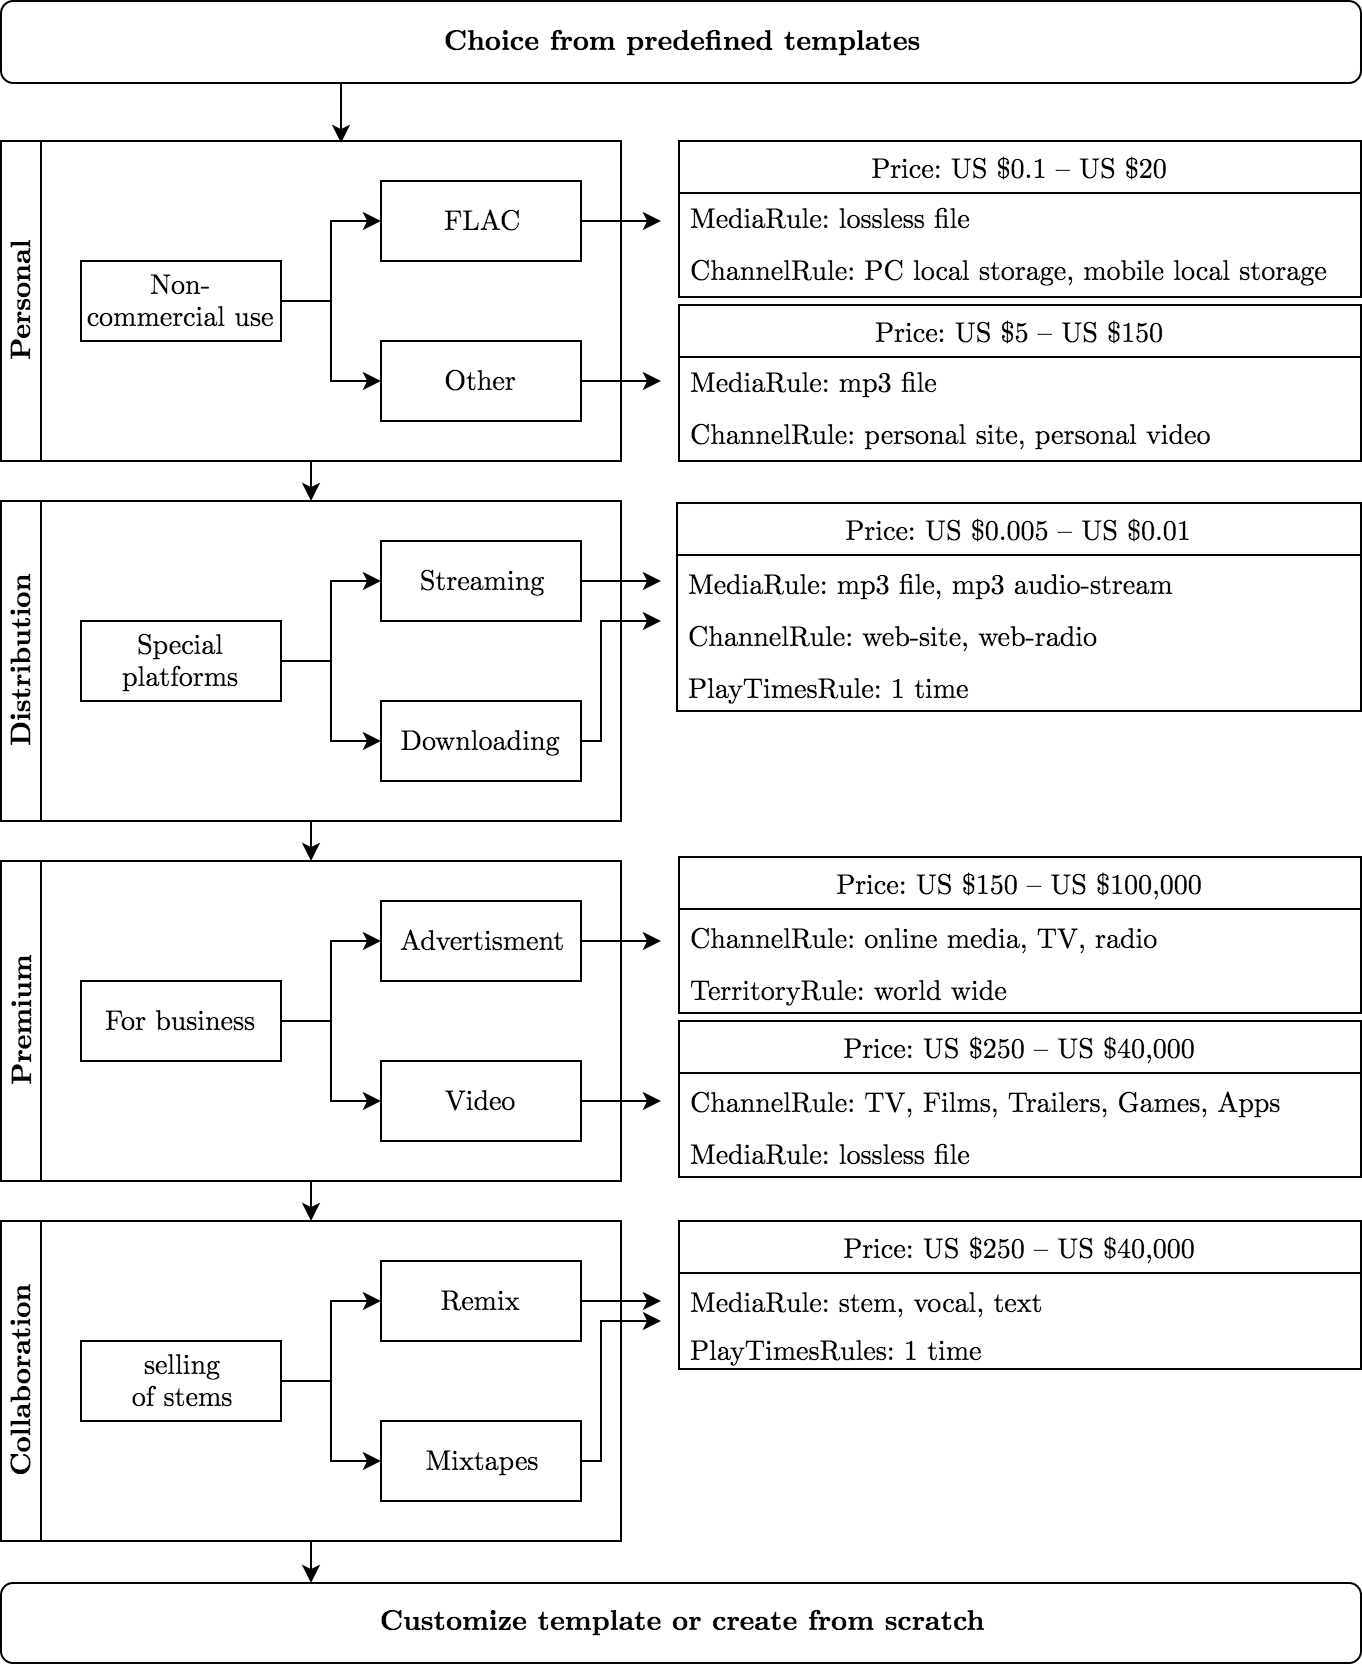
\includegraphics[width=\textwidth]{licensing}
\end{figure}

\begin{figure}[h]
\centering
\caption{Royalty Distribution}
\vspace{20pt}
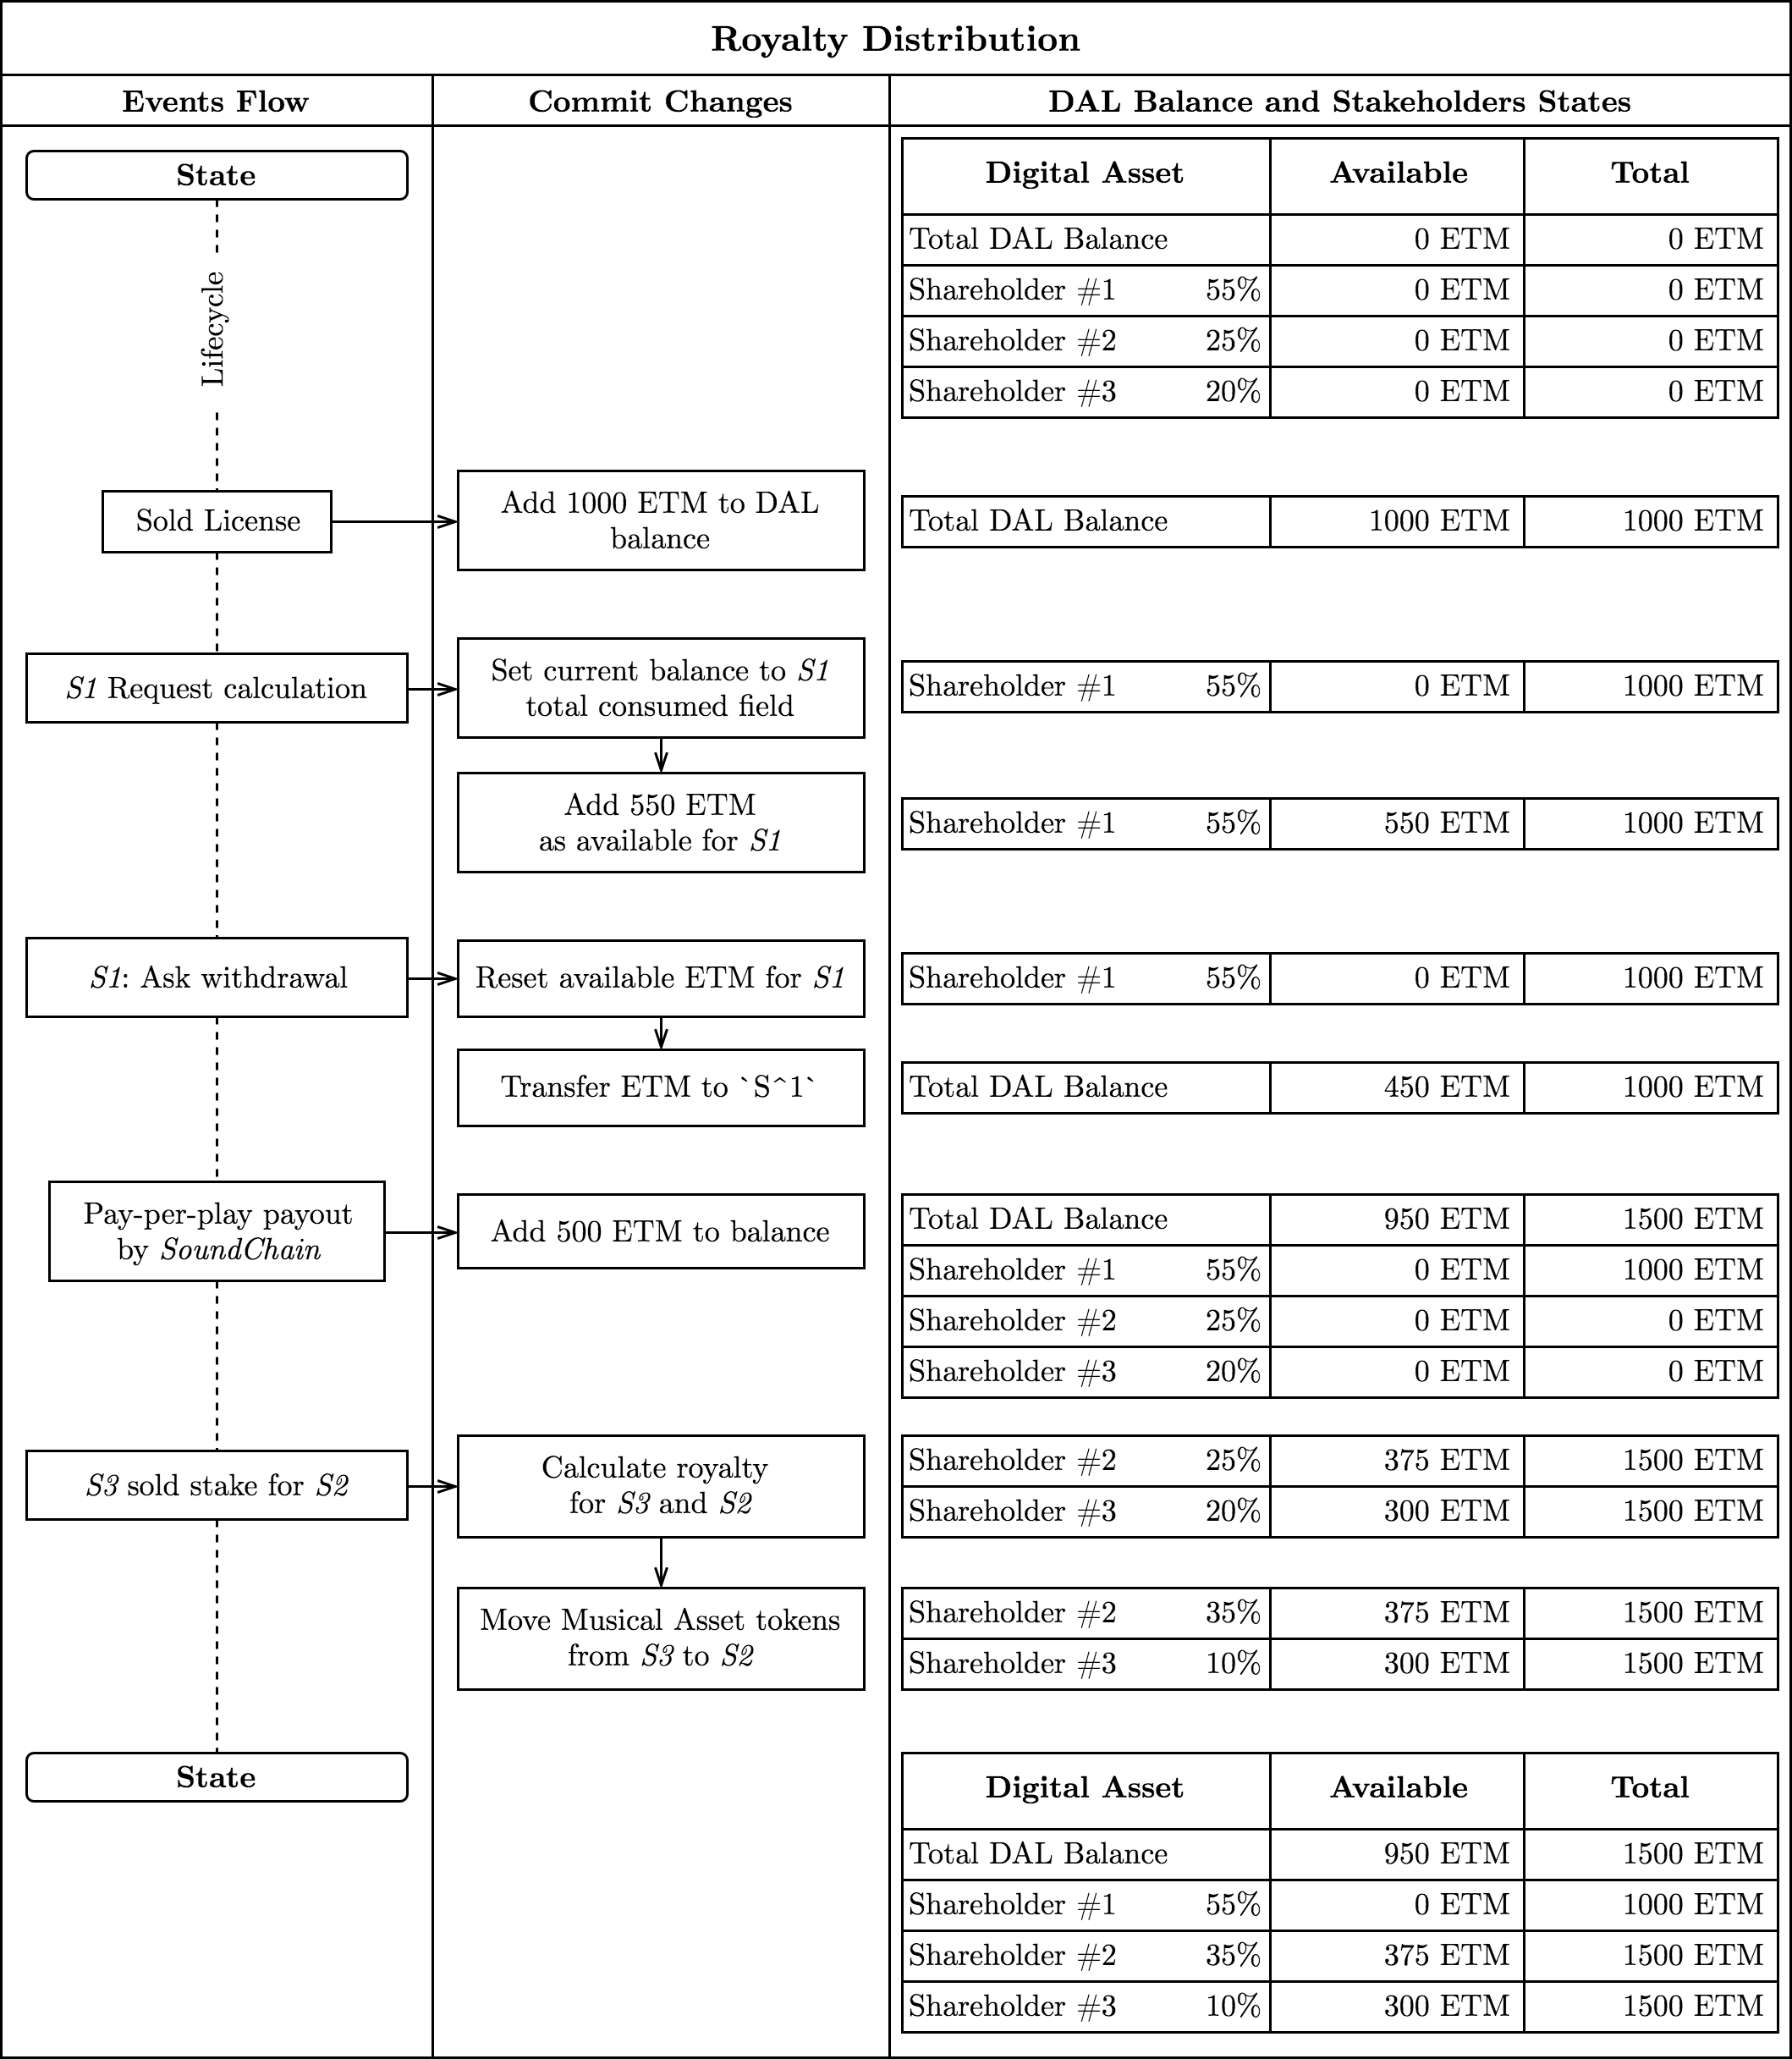
\includegraphics[width=\textwidth]{royalty}
\end{figure}
\section{Roles}
\label{platform-roles}
In a nature of platform users could identify yourself with desired roles as well as delegate roles to others.

Primary platform select next core roles:
\begin{itemize}
	\item \textbf{User} is the person who create an account on the platform and got permissions to hold and transfer ETM and interact with a musical catalog.
	\item \textbf{Person} is the user who provide proof-of-personality to receive permissions to invest and trade with a musical assets.
	\item \textbf{Artist} is a person with at least one registered musical asset on a platform. Should be at least person to register asset.
	\item \textbf{Notary} is the person chosen for the production of blocks
	\item \textbf{Affilated specialist} is the person chosen to do some important work for the platform. 
	\item \textbf{Keeper} is the user provided storage to store musical content.
\end{itemize}

\chapter{Technical Description of Platform}
\section{Overview}
\label{tech-review}
\begin{multicols}{2}
Musereum protocol tasks can be divided into the folllowing components:
\begin{itemize}
\item Providing unified system state without central computing for reliable operation;
\item Decentralized big data storage that is censor-proof due to inability to block a unified (centralized) data source;
\item Providing proof of system integrity for change history auditing;
\item Interface for making changes in the future state of the system.
\end{itemize}
\vfill\null
\columnbreak
Application of the "Blockchain concept" using Ethereum Virtual Machine (EVM) provides monitoring and changing single state of Musereum system without the need to use centralized computing (see \hyperref[tech-blockchain]{Blockchain} for detail). IPFS technology is applied to store big data volumes (audio tracks, metadata, text and graphical description) \textit{(see \hyperref[tech-storage]{Decentralized Storage} for more detail)}.

\end{multicols}
\pagebreak
\subsection{Naming convention}
\label{tech-review-naming}
\begin{multicols}{2}
Here and elsewhere all entities with defined content or interface will get a short mathematical name with a common rule: \textit{capital latin letter except for N, B, Z}, e. g:

\begin{equation}
Y \ \text{is Notary}
\end{equation}

All globally defined contracts will be assigned to a lowercase Greek symbol, e. g. Notary Registry Contract – $\nu$ and a special record associated with certain function of the contract:

\begin{equation}
\nu \ \text{is Notary Registry Contract}
\end{equation}
\begin{equation}
\nu_{vote} \ \text{is vote contract method}
\end{equation}
%\vfill\null
%\columnbreak

Sets of all known entities are defined as accepted entity name in a blackboard record except for $\mathbb{N}, \mathbb{B}, \mathbb{Z}$, e. g.: list of notaries:

\begin{equation}
\mathbb{Y} \ \text{is set of all known Notaries}
\end{equation}

$\mathbb{N}$ – set of all integers within the range $(0; 2^{256} - 1)$. $\mathbb{N}_1$ – subset $\mathbb{N}$ without 0.

$\mathbb{Z}$ – set of all integers within the range $(-2^{255}; +2^{255} - 1)$.

$\mathbb{B}$ – is a set of all bytes $(0; 255)$. 

$\mathbb{X}^{i}$ – is a set of dimension $i$ where every set member belongs to $\mathbb{X}$, e.g.:
\begin{equation}
\mathbb{B}^{32} \text{ is a set of } \mathbb{B} \text{ with size } 32
\end{equation}

Obtaining the set member can be described in two ways: with a subindex or in square brackets:
\begin{equation}
\begin{aligned}
\mathbb{Y}_2 = \mathbb{Y}[2] \\
\mathbb{Y}_n = \mathbb{Y}[n] 
\end{aligned}
\end{equation}

External data is represented in the formulae as members of set $\Gamma$with readable names (or abbreviations if mentioned), e. g.: Global time in UNIX format:
\begin{equation}
\Gamma_{time} \ \text{is world time variable}
\end{equation}

All \hlc{temporal} variables in formulae are written as latin letters, e. g.:
\begin{equation}
\begin{aligned}
\text{Let } a \text{ is a second notary in list of notaries} \\
a = \mathbb{Y}[2]
\end{aligned}
\end{equation}
\end{multicols}

\subsection{Mathematical functions and symbols}
\label{tech-review-math}
%\begin{multicols}{2}
All formulae apply $|\mathbb{Y}|$ as an operator of number of $\mathbb{Y}$-set elements.

The following conventions and functions are applied to reduce and/or make a mathematical notation readable:

\textbf{Search index in set} – $\mathcal{I}$:
\begin{align}
&\ \text{Let } a \text{ is a set of values: } \nonumber\\
a =&\ {100, 200, 300} \nonumber\\
f(v, x) =&\ \{i \ | \ i \in \mathbb{N},  i > |v|, v_i = x \} \\
\mathcal{I}(v, x) =&\ \begin{cases}
	min(f(v,x)), & \text{if } |f(v, x)| > 0 \\
	-1, & \text{overwise}
\end{cases}
\\
\\
r1 = &\ \mathcal{I}(a, 200) = 1\nonumber \\
r2 = &\ \mathcal{I}(a, 400) = -1
\end{align}

\textbf{\hlc{Determining} named tuple} – $\mathcal{O}$:
\begin{align}
&\ \text{Let } a \text{ is a set of names: } \nonumber\\
a =&\ \{name, age, height\} \nonumber\\
&\ \text{and let } b \text{ is a set of indexes: } \nonumber\\
b =&\ \{0, 1, 2\} = \{x \ | \ x \in \mathbb{N}, x < |a|\} \\
& \nonumber\\
&\ \text{finaly } r \text{ is a target named tuple, where} \nonumber\\
r =&\ \mathcal{O}(a) = \mathcal{O}(name, age, height) \\ 
r =&\ \{x_i \ | \ i \in  a, x_i = 0 \}
\end{align}

\textbf{\hlc{Determining} event tuple } – $\mathcal{E}$:\hfill\null\linebreak
Special defined tuple containing target data and general data for every event: \code{event}, \code{txHash}, \code{txIndex}, \code{blockHash}, \code{blockHeight}, \code{address}.
\begin{align}
&\ \text{Let } a \text{ is a set of default event fields: } \nonumber\\
a =&\ \{event, txHash, txIndex, blockHash, blockHeight, address\} \nonumber\\
&\ \text{Let } b \text{ is a set of extra event fields: } \nonumber\\
b =&\ \{asset, index\} \nonumber\\
&\ \nonumber\\
&\ \text{finaly } e \text{ is a target event tuple, where} \nonumber\\
r =&\ \mathcal{E}(b) \\
r =&\ \mathcal{O}(\{asset, index\} \ \cup \ a)
\end{align}
%\end{multicols}

\pagebreak
\section{Platform architecture}
\label{tech-arch}
\begin{multicols}{2}
The primary aim of the platform is to provide users with capabilities to:
\begin{enumerate}
\item Read and interpret data
\item \hlc{Commit} changes
\item Search data
\item Audit and receive proof of data \hlc{integrity}
\end{enumerate}
The platform is divided into the following logic layers in order to provide above-mentioned capabilities:
\begin{itemize}
	\item \hyperref[tech-arch-underlayer]{Storage and \hlc{ledger}}
	\begin{itemize}
		\item \hyperref[tech-blockchain]{Blockchain}
		\item \hyperref[tech-storage]{Decentralized storage}
	\end{itemize}
	\item \hyperref[tech-arch-connect]{Read and write \hlc{layer}}
	\begin{itemize}
		\item \hyperref[tech-arch-connect-nodes]{Public nodes}
		\item \hyperref[tech-arch-connect-validators]{Notary nodes}
	\end{itemize}
	\item \hyperref[tech-arch-interfaces]{Interaction interfaces}
	\begin{itemize}
		\item \hyperref[tech-arch-interfaces-dapp]{Decentralized application}
		\item \hyperref[tech-arch-interfaces-api]{Application Programming Interface}
	\end{itemize}
\end{itemize}
\end{multicols}

\def\Interface{Interaction Interface}
\def\Connect{Access layer}
\def\Underlayer{Storage and ledger layer}

\def\DApps{Decentralized Applications}
\def\Api{API}
\def\Requests{Direct \hlc{requests}}

\def\RPC{Musereum RPC}
\def\Nodes{Public nodes}
\def\Notaries{Notaries}
\def\EVM{Ethereum Virtual Machine}
\def\Blockchain{Blockchain ledger}
\def\IPFS{IPFS}
\def\ReadWrite{Read and write}
\def\ReadOnly{Read only}

\begin{center}
\begin{tikzpicture}[node distance=1.5cm]
\node (DApps) 					[rect]
										{\DApps};
\node (Api)						[rect, right=0.2cm of DApps]
										{\Api};
\node (Requests)				[rect, right=0.2cm of Api]
										{\Requests};
\node (Interface)				[above=0.5cm of DApps.north west, anchor=west] {\Interface};										

\node (InterfaceRect)		[rect, rounded corners, dashed, fit={(Interface) (DApps) (Api) (Requests)}] {};

\path 
	let \p1=(DApps.west), \p2=(Requests.east)
	in node(RPC) [
		rect,
		below=1.5cm of DApps.south west,
		anchor=north west,
		minimum width=\x2-\x1-\pgflinewidth
	] {\RPC};
    
\path 
	let \p1=(RPC.west), \p2=(RPC.east)
	in node(Nodes) [
		rect,
		below=0.4cm of RPC.south west,
		anchor=north west,
		minimum width=(\x2-\x1-\pgflinewidth)
	] {\Nodes};
    
\path 
	let \p1=(Nodes.west), \p2=(Nodes.east)
	in node(Notaries) [
		rect,
		below=1.8cm of Nodes.south west,
		anchor=north west,
		minimum width=(\x2-\x1-\pgflinewidth)/2-0.3cm
	] {\Notaries};
    
\draw 
	let \p1=(Nodes.south), \p2=(Notaries.north) 
	in [arrow] (\x2,\y1) -- node [fill=white] {\ReadWrite} (Notaries.north);
	
\draw [arrow] (RPC) -- (Nodes);

\node (Connect)			[above=0.5cm of RPC.north west, anchor=west] {\Connect};
\node (ConnectRect)		[rect, rounded corners, dashed, fit={(RPC) (Nodes) (Notaries) (Connect)}] {};

\draw [thick] (Nodes) -- node [fill=white, yshift=15pt]{\ReadOnly} (ConnectRect.south);

\path
	let \p1=(Nodes.west), \p2=(Nodes.east)
	in node(EVM) [
		rect, 
		below=1.5cm of Notaries.south west,
		anchor=north west,
		minimum width=(\x2-\x1-\pgflinewidth)/2-0.1cm
	] {\EVM};
	
\path
	let \p1=(Nodes.west), \p2=(Nodes.east)
	in node(Blockchain) [
		rect, 
		below=0.4cm of EVM.south west,
		anchor=north west,
		minimum width=(\x2-\x1-\pgflinewidth)/2-0.1cm
	] {\Blockchain};
\path
	let \p1=(Nodes.west), \p2=(Nodes.east),
	     \p3=(EVM.north), \p4=(Blockchain.south)
	in node(IPFS) [
		rect, 
		below=0pt of EVM.north east,
		anchor=north west,
		xshift=0.2cm,
		minimum width=(\x2-\x1-\pgflinewidth)/2-0.1cm,
		minimum height=(-\y4+\y3)
	] {\IPFS};
\node (Underlayer)			[above=0.5cm of EVM.north west, anchor=west] {\Underlayer};
\node (UnderlayerRect)		[rect, rounded corners, dashed, fit={(EVM) (Blockchain) (IPFS) (Underlayer)}] {};
    
\draw [arrow] (EVM) -- (Blockchain);
\draw [arrow] (InterfaceRect) -- (ConnectRect);
\draw [arrow] (ConnectRect) -- (UnderlayerRect);
\end{tikzpicture} 
\end{center}

\subsection{Storage and record layer}
\label{tech-arch-underlayer}
\begin{multicols}{2}
Storage and record layer is the basic layer of the platform. The layer provides capability to keep a decentralized state ledger (blockchain) and to store big amounts of data.

Every layer element: blockchain, storage and virtual machine are distributed among the network (nodes) and everyone can create a personal local copy.
\end{multicols}
\subsection{Access layer}
\label{tech-arch-connect}
\begin{multicols}{2}
Access layer application: providing data from the basic layer on request and receiving change requests.

Creating a node for an additional access point is not limited and available for anyone. This feature is a benefit that distinguishes Musereum platform from other centralized music platforms:

\begin{itemize}
	\item It provides 100\% network up-time
	\item It is Censor-proof
	\item Stakeholders can create a personal local copy of the network without necessity to trust third parties
\end{itemize}
\end{multicols}
\pagebreak
\subsection{Interaction interface layer}
\label{tech-arch-interfaces}
\begin{multicols}{2}
Interaction interface layer is the top layer of the platform. The layer receives user input and generates requests applicable with protocol. Requests are divided into two types: read and write.

Reading data from the blockchain and the decentralized storage is not limited. The only requirement is to form a request according to API agreement.

In order to write (changing state, saving data), a user must provide valid request signature based on his or her unique private key as well as follow other writing requirements (rights, funds for protocol operation etc.).

It is not required for an organization to have its own access point (synchronize a node with the network) in order to make a request; a serverless web-application can be used as a client \textit{(see \hyperref[tech-apps]{Decentralized applications} for detail)}.

\end{multicols}
\section{Blockchain}
\label{tech-blockchain}
\begin{multicols}{2}
Musereum protocol is an open public blockchain that requires permission to generate blocks and is based on Ethereum protocol. Consensus for a single network state in a decentralized block generator structure is achieved by Proof-of-Authority (hereafter PoA) algorithm. Achieving consensus through PoA requires:
\begin{enumerate}
\item A common list of notaries ($\mathbb{Y}$) permitted to generate blocks;
\item Notary Registry Contract ($\nu$).
\end{enumerate}
The list of notaries can be changed (excluding / appointing notaries) by Notary Registry Contract based on results of active notary voting (majority).

\textit{Initially, 12 notaries are listed.}

Notary \hlc{duties}: 
\begin{enumerate}
\item Validate transactions received from system participants,
\item \hlc{Write changed state to a new block},
\item \hlc{Sign block chain} with a personal crypto-signature.
\end{enumerate}

In order to maintain consensus, an external constant $\Gamma_{step}$ is introduced, it defines the number of seconds in one time step or time between blocks. Musereum defines constant $\Gamma_{step}$ as 5 or 1 block every five seconds.
\begin{equation}
\Gamma_{step} = 5
\end{equation}
According to PoA consensus algorithm, a notary has the right to generate one block ($K$) in $a$ \hlc{timestamps} $\Gamma_{time}$. If $a$ is a number of notaries:
\begin{equation}
a = |\mathbb{Y}|
\end{equation}
Notary index $i$ is selected from set $\mathbb{Y}$ to create a block on time stamp $b$according to the formula: 
\begin{equation}
b = \frac{\Gamma_{time}}{\Gamma_{step}},  \quad b \in \mathbb{N} 
\end{equation}
\begin{equation}
i = b \ mod \ a
\end{equation}
\end{multicols}
\subsection{Version selection}
\label{tech-blockchain-score}
%\begin{multicols}{2}
In case if notaries fail to achieve global (single) system state and a fork or creating two or more blockchains takes place ($\mathbb{K}$), the network defines the score ($\beta_{score}(\mathbb{K}_c)$) of every  chain based on the number of notaries participating in \hlc{chain creation}:	
%\vfill\null\columnbreak
\begin{align}
h &= |\mathbb{K}_c| & \quad h \ \text{is length of blockchain} \\
\beta_{score}(\mathbb{K}_c) &= \Gamma_{u128max} * h - m
\end{align}
The network always selects the chain with the highest score according to $\beta_{score}$.
%\end{multicols}
\subsection{Block finalization}
\label{tech-blockchain-fin}
% \begin{multicols}{2}
According to consensus, the block in the chain after which more than 50\% of notaries have generated 2 or more blocks is considered irreversable.

Thus, the minimal time for complete block validation ($C$) is:
\begin{equation}
C = 2 * \Gamma_{step} * |\mathbb{Y}|
\end{equation}
\textit{Or 120 seconds with default protocol settings: 12 notaries with 1 block every five seconds}
% \end{multicols}
\subsection{Notary Witness}
\label{tech-blockchain-confirmation}
\begin{multicols}{2}
In order to do any activity that requires changing system state, user must form a transaction ($T$) signed with a unique cryptographic signature ($T_{sign}$). 

The crypto-signature is a warrant for the network that proves owner's will to create a transaction using creator's account. 

The notary in turn to generate a block checks the validity of a transaction and executes the related code:
\begin{enumerate}
\item Sender has the right to create a transaction for the given address – $\rho_{allowTx}(T_{from}, T_{to})$ \textit{(see \hyperref[tech-blockchain-rules]{EVM Interaction Rules} for detail)}
\item Transaction meets formal criteria – $\rho_{initialValid}(T)$
\item Checking account owner's signature – $\rho_{checkSign}(T)$
\item Checking sufficient amount of tokens on ETM account to pay in advance for computer operation – $\rho_{upFront}(T)$
\item Execution of related	EVM code	did not 	throw an exception $\rho_{exception}(\rho_{execute}(T))$
\end{enumerate}
\end{multicols}
\begin{align}
\rho_{success}(T) = 	&\rho_{allowTx}(T_{from}, T_{to}) &> 0 \ \wedge \\
 								&\rho_{initialValid}(T) &> 0 \ \wedge \\
								&\rho_{checkSign}(T) &> 0 \ \wedge \\
								&\rho_{upFront}(T) &> 0 \ \wedge \\
 								&\rho_{exception}(\rho_{execute}(T)) &= 0
\end{align}
\begin{multicols}{2}
Having validated the transaction, notary packs the transaction in blocks and informs the network about the block and change of the network state ($\mathbb{W}_h$).
\begin{equation}
\mathbb{W}_h = \rho_{state}(\mathbb{W}_{h-1}, \mathbb{K}_h)
\end{equation}
Other notaries receive the block, check it ($\rho_{success}(T)$) and take decision to accept it to the chain. By creating a block on $\mathbb{K}_h$ the notary validates the block and all included transactions.
Thus, the transaction may have from 1 to $|\mathbb{Y}|$ validating signatures.
Minimal time for receiving $|\mathbb{Y}|$ signatures:
\begin{equation}
a = \Gamma_{step} * |\mathbb{Y}|
\end{equation}
\end{multicols}
\vfill\null\pagebreak

\subsection{Crosschain communication and Ethereum Classic}
\label{tech-blockchain-anchoring}
\begin{multicols}{2}
В целях повышения безопастности и отказоустойчивости сети, Musereum периодически дублирует ключевую информацию о состоянии сети и событиях во внешний неконтролируемый нотариусами блокчейн. 

В качестве блокчейна для хранения ключевой информации выбрана сеть Ethereum Classic, по следующим причинам:
\begin{itemize}
	\item Общая капитализация сети – \$1,811,306,656
	\item Стоимость атаки 51\% на сеть составляет более \$40,000,000
	\item Permission-less консенсус – PoW.
\end{itemize}

Musereum публикует в Ethereum Classic:
\begin{enumerate}
	\item хеши каждого n блока для обеспечения доказательства исторических данны;
	\item факты ключевых сделок: регистрация музыкальных активов, покупка лицензий.
\end{enumerate}
\end{multicols}

\begin{figure}[h]
\centering
\caption{Crosschain communication}
\vspace{20pt}
\begin{tikzpicture}
\tikzset{%
	part/.style = { rectangle, draw=black, minimum height=.7cm },
	block/.style = { rectangle, draw=black, minimum height=3cm, minimum width=3cm, text width=3cm, text centered},
	event/.style = { rectangle, , rounded corners, draw=black, text centered},
	anchoring/.style = { rectangle, rounded corners, draw=black, text centered, minimum width=3cm, minimum height=1.2cm}
}
\node(BlockA)			[block]
								{Musereum \linebreak Block};
\node(BlockB)			[block, right=0.8cm of BlockA.east]
								{Musereum \linebreak Block};
\node(BlockC)			[block, right=0.8cm of BlockB.east]
								{Musereum \linebreak Block};
\node(BlockD)			[block, right=0.8cm of BlockC.east]
								{Musereum \linebreak Block};
								
\node(NewAsset)		[part, below=0.2cm of BlockB.south]
								{Asset Registration};
\node(BuyLicense)	[part, below=0.2cm of BlockC.south]
								{Buy License};
\node(StateHash)		[part, below=0.2cm of BlockD.south]
								{$K_{stateHash}$};
\node(StorageHash)	[part, below=0.2cm of StateHash.south]
								{$K_{storageHash}$};
\node(ReceiptHash)	[part, below=0.2cm of StorageHash.south]
								{$K_{receiptHash}$};
						
								
\node(ETCA)				[block, below=5.1cm of BlockA.south]
								{ETC Block};
\node(ETCC)				[block, below=5.1cm of BlockD.south]
								{ETC Block};			
\node(ETCB) 			[block] at ($(ETCA)!0.5!(ETCC)$) 
								{ETC Block};

\node(AnchoringA)	[anchoring,  below=3.1cm of BlockB.south]
								{Anchor Contract};
								
\node(AnchoringB)	[anchoring,  below=3.1cm of BlockD.south]
								{Anchor Contract};


%\draw[->] (manufacturer.south) -- ++(-.5,0) -- ++(0,-1) -|  (retailer1.north);	
%\draw[myarrow] (manufacturer.south) -- ++(.5,0) -- ++(0,-1) -|  (retailer2.north);

\draw [line]		(BlockB) -- (NewAsset);
\draw [arrow]	(NewAsset) 	-- (AnchoringA);
\draw [arrow] 	(AnchoringA) -| (ETCB);

\draw [line]		(BlockD) --	
						(StateHash) --
						(StorageHash) -- 
						(ReceiptHash);
						
\draw [line	]		(BlockC) -- (BuyLicense);
						
\draw [arrow] 	(ReceiptHash) 	-- 	(AnchoringB);
\draw [arrow] 	(BuyLicense)		|- 	(AnchoringB);
\draw [arrow] 	(AnchoringB)		-- 	(ETCC);


\draw [vecArrow] 	(BlockD) -- (BlockC);
\draw [vecArrow] 	(BlockC) -- (BlockB);
\draw [vecArrow] 	(BlockB) -- (BlockA);
\draw [innerWhite](BlockD) -- (BlockC);
\draw [innerWhite](BlockC) -- (BlockB);
\draw [innerWhite](BlockB) -- (BlockA);

\draw [vecArrow] 	(ETCC) -- (ETCB);
\draw [vecArrow]	(ETCB) -- (ETCA);
\draw [innerWhite](ETCC) -- (ETCB);
\draw [innerWhite](ETCB) -- (ETCA);
							
\end{tikzpicture}
\end{figure}

\vfill\null\pagebreak

\subsection{Block Generation Reward}
\label{tech-blockchain-reward}
\begin{multicols}{2}
Block reward ($R$) consists of two parts: new emission and activity fees.

Musereum platform implies emission of new ETM tokens by creation of a block. Emission is limited to 3 ETM per block.

Amount of activity fee is calculated independently for each transaction. The sender indicates in transaction difficulty unit price ($T_{gasPrice}$) that he or she is ready to spend to compensate network operation.

Final 	fee is calculated according to formula:
\begin{equation}
x = T_{gasPrice} * \rho_{dificulty}(\rho_{execute}(T))
\end{equation}

Total block reward:
\begin{align}
&\text{Let } a \text{ is a list of transactions of block } \mathbb{K}_h \\
a &= \mathbb{K}[h]_{transactions} \\
\mathbb{R}_h &= 3 + \sum\limits_{i=0}^{|a|} a_i
\end{align}
\end{multicols}

\subsubsection{Reward distribution}
\label{tech-blockchain-reward-distribution}
Apart from Ethereum and Bitcoin protocols, Musereum network has no miners – the primary value is created by artists who select Musereum platform for publication and distribution of music.

Musereum highly appreciates artitsts' contribution to platform integrity and it sends the most part of block reward to fund artists.

General distribution pattern:

\def\Musereum{Musereum}
\def\Development{Platform Development}
\def\Infrastructure{Infrastructure}

\begin{figure}[h]
\centering
\caption{Block reward distribution}
\vspace{20pt}
\begin{tikzpicture}[scale=3]

\newcounter{c}
\newcounter{d}
\foreach \p/\t in {
	80/\Musereum,
	10/\Development, 
	10/\Infrastructure}
  {
    \setcounter{c}{\value{d}}
    \addtocounter{d}{\p}
    \slice{\thec/100*360}
          {\thed/100*360}
          {\p\%}{\t}
  }

\end{tikzpicture}
\end{figure}

\begin{itemize}
	\item 80\% – Musereum:
	\begin{itemize}
		\item 90\% – SoundChain Trust \textit{(see more in \hyperref[tech-apps-soundchain-payperplay]{Pay-per-Play})}
		\item 10\% – bounty programs: Fans Bounty, Clipmaker Bounty and etc.
	\end{itemize}
	\item 10\% – Platform Development Foundation
	\item 10\% – \hlc{Network Infrastructure}
	\begin{itemize}
		\item 25\% – Notaries / Validators
		\item 25\% – \hlc{Keepers}
		\item 25\% – Affilated specialists (\hlc{registrators} and smart-contract auditors)
		\item 25\% – Oracles
	\end{itemize}
\end{itemize}


\subsection{Ethereum VM}
\label{tech-blockchain-evm}
Ethereum is an open-source, public, blockchain-based distributed computing platform featuring smart contract (scripting) functionality. It provides a decentralized Turing-complete virtual machine, the Ethereum Virtual Machine (EVM), which can execute scripts. "Gas", an internal transaction pricing mechanism, is used to mitigate spam and allocate resources on the network.
\subsection{Ethereum Smart-contracts}
\label{tech-blockchain-contracts}
Smart contracts are deterministic exchange mechanisms controlled by digital means that can carry out the direct transaction of value between untrusted agents. They can be used to facilitate, verify, and enforce the negotiation or performance of economically-laden procedural instructions and potentially circumvent censorship, collusion, and counter-party risk. In Ethereum, smart contracts are treated as autonomous scripts or stateful decentralized applications that are stored in the Ethereum blockchain for later execution by the EVM. Instructions embedded in Ethereum contracts are paid for in ether (or more technically "gas") and can be implemented in a variety of Turing complete scripting languages.
\subsection{Musereum rules for EVM interaction}
\label{tech-blockchain-rules}
%\begin{multicols}{2}
In order to improve security of platform participants, interaction with EVM smart contracts in Musereum differs from that in parental Ethereum network.

Any member of the network can upload a smart contract to the network, but such smart contract has $P_{development}$ status and it is available for interaction with affiliated addresses of network accounts. Initially this address belongs to the account of the user who uploaded the contract.

Smart contract interaction rules are regulated by allowance smart contract: $\rho$.

Any smart contract call initially requests allowance to make the call – $\rho_{allowTx}(T_{from}, T_{to})$
%\end{multicols}
\begin{align}
a &= \rho_{stateOf}(T_{to}) \nonumber\\
b &= \rho_{affilateWith}(T_{to}) \nonumber\\
\rho_{allowTx}(T_{from}, T_{to}) &= \begin{cases}1, & \text{if } a = P_{production} \\ 1, & \text{if } a = P_{development} \wedge T_{from} \in b \\ 0, & \text{overwise} \end{cases}
\end{align}
The author of a smart contract must provide source code for a check and pass the checking procedure in order to get $P_{production}$ status \textit{(see for details \hyperref[tech-apps-contracts-registry]{Smart Contract Registry})}

% Nodes
\def\Owner{Владелец контракта}
\def\Blockchain{Блокчейн}
\def\Registry{Реестр контрактов}
\def\LoadByteCode{Uploading byte code to blockchain}
\def\LoadSourceCode{Uploading source code}
\def\ValidationEnded{Code \hlc{Validation is} passed?}
\def\ChangeStatus{Changing smart contract state}

\begin{center}
\begin{tikzpicture}[node distance=1.5cm]
\node (LoadByteCode)		[rect, text width=11.5em] 
										{\LoadByteCode};

\node (LoadSourceCode)	[rect, text width=11.5em, below of=LoadByteCode] 
										{\LoadSourceCode};

\node (ValidationEnded)	[event, text width=11.5em, below=1.5cm of LoadSourceCode]
										{\ValidationEnded};
										
\node (aux0)[right=2cm of ValidationEnded]{};
\node (Invalid)					[text width=5em, above of=aux0]
										{$\pi_{ended} = 0$};

\node (ChangeStatus)		[rect, text width=11.5em, below of=ValidationEnded]	
										{\ChangeStatus};

\node (InDevelopment)		[inout, text width=11em, right=1cm of LoadByteCode]			
										{$\rho_{stateOf}(a) = P_{development}$};
										
\node (InProduction)			[inout, text width=11em, right=1cm of ChangeStatus]			
										{$\rho_{stateOf}(a) = P_{development}$};

%arrows
\draw [arrow] (LoadByteCode)				-- (LoadSourceCode);
\draw [-, thick, dashed]
	(LoadByteCode)								--(InDevelopment);
\draw [arrow] (LoadSourceCode) 			-- (ValidationEnded);
\draw [arrow] (ValidationEnded)			-- (ChangeStatus);
\draw [arrow] (ValidationEnded)			-| (Invalid);
\draw [thick]  (Invalid)  							-| (ValidationEnded);
\draw [-, thick, dashed] 
	(ChangeStatus)									-- (InProduction);

\end{tikzpicture} 
\end{center}

\section{Decentralized Storage}
\label{tech-storage}
\subsection{Overview}
\label{tech-storage-review}
\textit{InterPlanetary File System} (IPFS) is a peer-to-peer network connecting remote servers in a single global decentralized storage platform. A significant amount of storage capacity will be required to store all the compositions in a decentralized manner and this can be achieved through IPFS.

Musereum is planning to utilize customized Clustered IPFS Swarm for the platform. Clustered IPFS nodes should create the necessary storage capacity for storing beats, compositions and videos, while providing faster access to them. Files stored in IPFS are divided into smaller chunks and each chunk is encrypted with keys. Based on our experience, storing files as chunks can significantly reduce download time and make them more secure.

The Musereum community will be involved in storing and streaming of the compositions and gain rewards in return from emission rate of ETM tokens.
\subsection{Naming System}
\label{tech-storage-naming}
Musereum is planning to utilize \textit{The Inter-Planetary Naming System} (IPNS) to provide simple way to stored files. 

It allows you to store a reference to an IPFS file under the namespace of corresponding KeeperID (the hash of keeper's public key).

\section{Децентрализованные приложения}
\label{tech-apps}
Musereum DApps implement the code for record and storage layer as well as the interaction interface code. The protocol allows DApps to interact.

\subsection{Governance dApp}
\label{tech-apps-governance}
\begin{multicols}{2}
Musereum starts from initial ceremony to set up a list of Notaries.

During the initial ceremony a master of ceremony creates a set of keys for each validator. He/She distributes them to validators one by one. Before each distribution of keys, he/she sends a transaction to a smart contract with a list of validators. That smart contract is used by consensus algorithm to determine if a validator has rights to participate in consensus and create blocks. The validator’s smart contracts are used by other DApps, e.g. Governance DApp and Payout DApp.

A validator generates three keys in the Initial Ceremony DApp:
\begin{itemize}
	\item mining key, required to participate in consensus and create blocks.
	\item voting key, required to create ballots and vote on ballots.
	\item payout key, not required. Used in Payout DApp to send daily mined coins from the mining key to the payout key. If a mining node should be compromised, an attacker will get daily earnings or less.
\end{itemize}

All keys are generated on the client side and not transmitted over the Internet without a validator’s permission and willingness. When keys are generated, the validator stores them on secure local storage, e.g. saves them to a hardware wallet and the password to a password manager. The validator signs a transaction to the validator’s contract with the initial key, provided by the master of ceremony.

Initial ceremony is a required procedure to start a new network based on Oracles Network’s ideas of independent validators.
\end{multicols}

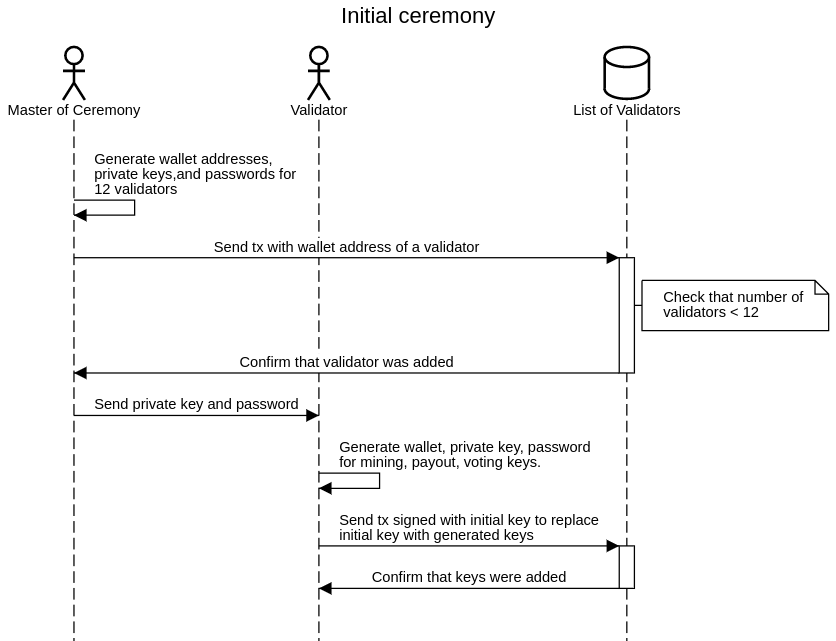
\includegraphics[width=\textwidth]{initial}

\begin{multicols}{2}
Futurе changes of Notaries List will be committed through voting. Creation of voting ballot based on a request with assign form.

Valid notary of the Oracles Network fills out a form in DApp providing:
\begin{itemize}
	\item mining key - mining key of a new or existing notary, which will be voted on
affected key type - key type (mining, payout, or voting key) of a new or existing notary, which will be voted on
	\item memo - brief information about notary, which will be voted on
	\item action - add affected key to the network or remove it from the network
\end{itemize}

If the affected key type is mining key, the user will be asked to provide personal data of the notary (owner of this mining key) such as full name, physical address, U.S. state name, zip code, notary license ID, and notary license expiration date.

At the final step, one transaction to create a new ballot in Oracles contract will be pushed to the blockchain to add a new ballot after the user presses “Continue” button. It should be noted, that in case of a mining key, it will be two consistent transactions: to add personal data of a notary and a new ballot to contract. User will see MetaMask popups equal to the number of transactions. After the confirmation and successful mining of the transaction by existing validators, the user will see the created ballot in the list and be able to vote on it. 
\end{multicols}

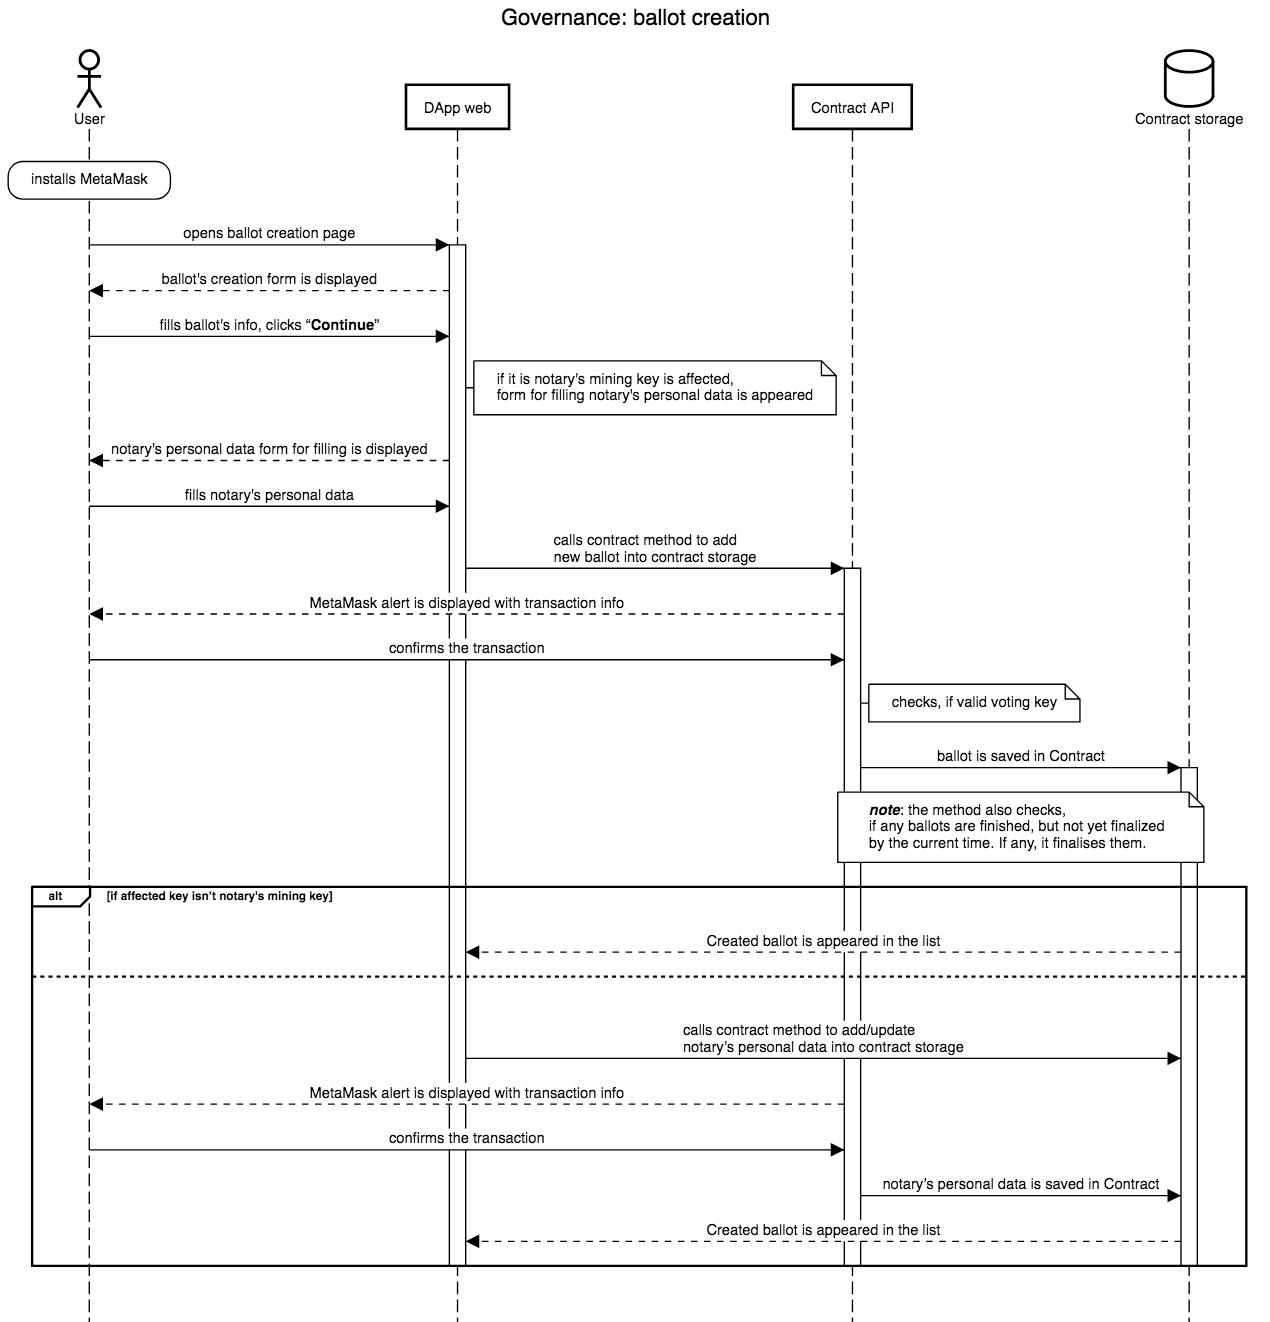
\includegraphics[width=\textwidth]{creation-ballot}

\subsection{Contract Registry}
\label{tech-apps-contracts-registry}
\begin{multicols}{2}
The DApp for registering and recording smart contracts of the platform.

The DApp smart contract allows to receive:
\begin{enumerate}
	\item The list of all registered smart contracts
	\item Smart contract state associated with the address:
	\begin{enumerate}
		\item \code{Unknown} – unknown state (default for unknown addresses in \hlc{Contract Registry })
		\item \code{Development} – smart contract is registered but currently is under development (interaction is allowed for affiliated users only)
		\item \code{Production} – smart contract is registered and \hlc{ready to interact}
		\item \code{Halt} – smart contract is registered but halted (by author's decision)
		\item \code{Suspend} – smart contract is registered but suspended (by auditor's decision)
	\end{enumerate}
\item A link to a source code repository
\item A link to ABI JSON for smart contract interaction
\item The list of affiliated auditors
\item A ballot \hlc{instance} to take decision about changing the state \textit{(see \hyperref[tech-apps-voting]{VotingDApp} for detail)}
\end{enumerate}
\end{multicols}
\subsubsection{Source code and smart contract checking}
\label{tech-apps-contracts-validate}
\begin{multicols}{2}
Smart contracts are validated in three ways:
\begin{itemize}
	\item Source code validation for:
		\begin{enumerate}
			\item Vulnerabilities 
			\item Compliance with stated business logic
			\item Absence of algorithmic errors
		\end{enumerate}
	\item Compliance with law applicable to Musereum platform
	\item Compliance with Musereum concept
\end{itemize}
\vfill\null
\columnbreak
In order to approve a smart contract, all affiliated auditors must have a unanimous consent for all three points.

Validation process can be monitored in \hyperref[tech-apps-voting]{Voting dApp} in corresponding\code{ContractValidationBallot}.
\end{multicols}
\subsection{Musereum Name System (MNS)}
\label{tech-apps-mns}
\begin{multicols}{2}
The Ledger of names associated with addresses in Musereum platform is required to provide access to up-to-date protocol apps avoiding the necessity to remember the internal address (20-character hex-address).

Name record can be created by any network user for a random address. Number of names for the address is unlimited.

In order to protect names from improper use, the registration of a new name is charged in ETM according to the current price.

Name record is a MNS-derived smart contract: \code{NameRecordContract}.

The smart contract contains the data about the name owner and associated network address and provides the following capabilities:
\begin{itemize}
	\item for the owner to change the associated address;
	\item for the owner to change the owner (transfer of right)
\end{itemize} 

MNS limits available names: 
\begin{itemize}
	\item Name length cannot exceed 20 characters (or less if non-ASCII characters are used) 
	\item Name length cannot be shorter than 4 characters
\end{itemize}
\end{multicols}
\subsubsection{Interaction interface}
\label{tech-apps-mns-api}
\code{mapping (address => address) names} – ($\eta_{names}$)\hfill\null\linebreak
List of addresses associated with addresses of name registration smart contracts

\code{uint price} – ($\eta_{price}$)\hfill\null\linebreak
Name registration price in ETM tokens

\code{event NewName(address indexed name, byte20 ascii)} – ($\eta_{NewName}$)\hfill\null\linebreak
\hlc{Event log} of new name registration

\code{event AssociateWith(address indexed name, address indexed target)} – ($\eta_{AssociateWith}$)\hfill\null\linebreak
Event log of address associating with name registration smart contract

\code{function buyName(byte20 acsii) payable} – ($\eta_{buy}$)\hfill\null\linebreak
Method to buy name. Returns \code{address} if the buying is successful and \code{throw} in case of error.

\begin{equation}
\eta_{buy}(s) = \begin{cases}
	throw, & \text{if } s \in \eta_{NewName} \\ 
	throw, & \text{if } |s| < 4 \\
	throw, & \text{if } T_{value} < \eta_{price} \\
	address, & \text{overwise}
\end{cases}
\end{equation}

\paragraph{Smart-contract NameRecord}– ($\eta'$)

\code{address owner} – ($\eta'_{owner}$)\hfill\null\linebreak
Current name owner

\code{byte20 ascii} – ($\eta'_{ascii}$)\hfill\null\linebreak
Registered name (typicaly is 20 ASCII letter)

\code{address target} – ($\eta'_{target}$)\hfill\null\linebreak
Current association with address on Musereum platform

\code{function associate(address target)} – ($\eta'_{associate}$)\hfill\null\linebreak
Change name association to the new address. Returns \code{true} if successful and \code{throw} in case of error.
 
\begin{equation}
\eta'_{associate}(a) = \begin{cases}
	throw, & \text{if } T_{from} \neq \eta'_{owner} \\
	throw, & \text{if } a = 0 \\
	true, & \text{overwise}
\end{cases}
\end{equation}

\subsection{Voting dApp}
\label{tech-apps-voting}
\begin{multicols}{2}
Voting DApp consists of connected elements:
\begin{itemize}
	\item \code{BallotsManager} ($\phi$)\hfill\null\linebreak
	Ballots registry
	\item \code{Ballot} ($\pi$)\hfill\null\linebreak
	Abstract voting smart-contract
	\item \code{VotingRightsToken} ($\phi^\tau$) \hfill\null\linebreak
	Token issued to voting participants to prove the voting right
	\item \textbf{Voting \hlc{GUI}}\hfill\null\linebreak
	\hlc{Web interface to interact with a ballots}
\end{itemize}
\vfill\null\columnbreak
In order to create a voting, the offer initiator must create a valid \code{Ballot}– a smart contract counting the votes and implementing \code{applyProposal} method to change the state based on the offer.
 
\end{multicols}

\begin{center}
\begin{tikzpicture}[node distance=1.5cm]
\node (LoadByteCode)		[rect, text width=11.5em] 
										{\LoadByteCode};

\node (LoadSourceCode)	[rect, text width=11.5em, below of=LoadByteCode] 
										{\LoadSourceCode};

\node (ValidationEnded)	[event, text width=11.5em, below=1.5cm of LoadSourceCode]
										{\ValidationEnded};
										
\node (aux0)[right=2cm of ValidationEnded]{};
\node (Invalid)					[text width=5em, above of=aux0]
										{$\pi_{ended} = 0$};

\node (ChangeStatus)		[rect, text width=11.5em, below of=ValidationEnded]	
										{\ChangeStatus};

\node (InDevelopment)		[inout, text width=11em, right=1cm of LoadByteCode]			
										{$\rho_{stateOf}(a) = P_{development}$};
										
\node (InProduction)			[inout, text width=11em, right=1cm of ChangeStatus]			
										{$\rho_{stateOf}(a) = P_{development}$};

%arrows
\draw [arrow] (LoadByteCode)				-- (LoadSourceCode);
\draw [arrow] (LoadByteCode)				-- (InDevelopment);
\draw [arrow] (LoadSourceCode) 			-- (ValidationEnded);
\draw [arrow] (ValidationEnded)			-- (ChangeStatus);
\draw [arrow] (ValidationEnded)			-| (Invalid);
\draw [thick]  (Invalid)  							-| (ValidationEnded);
\draw [arrow] (ChangeStatus)				-- (InProduction);

\end{tikzpicture} 
\end{center}

\subsubsection{Смарт-контракт Ballot}
\label{tech-apps-voting-ballot}
\begin{multicols}{2}
An abstract smart contract describing the requirements for final implementation of voting offers.

\code{address votingToken} – ($\pi_{token}$)\hfill\null\linebreak
A voting-associated token providing the holder with the voting right.

\code{function vote(bool)} – ($\pi_{vote}$)\hfill\null\linebreak
External method to write the decision requesting the method.

\code{function applyProposal()} – ($\pi_{apply}$)\hfill\null\linebreak
Abstract application method based on the successful voting. It is implemented in child smart contracts.

\code{uint agreeVotesCount} – ($\pi_{agree}$)\hfill\null\linebreak
Number of tokens transferred for accepting the decision.

\code{uint rejectVotesCount} – ($\pi_{reject}$)\hfill\null\linebreak
Number of tokens transferred for rejecting the decision.

\code{uint endTime} – ($\pi_{end}$)\hfill\null\linebreak
Voting ending time.

\code{function isEnded()}  - ($\pi_{ended}$)\hfill\null\linebreak
Returns 1 if voting time is over and 0 in other cases.
\begin{equation}
\pi_{ended} = \begin{cases}
	1, & \text{if } \pi_{end} > \Gamma_{time} \\
	0, & \text{overwise}
\end{cases}
\end{equation}

\code{function voteMajorityRule()} – ($\pi_{rule}$)\hfill\null\linebreak 
\hlc{Result of function} $f(x) = 1/x$ where $x$ is the ratio of "for" votes to total number of votes sufficient for accepting the decision:
\begin{equation}
\pi_{rule} = \begin{cases}
	\infty, & \text{if } x = 0 \\
	\frac{1}{x}, & \text{overwise}
\end{cases}
\end{equation}

\code{function compare()} – ($\pi_{compare}$)\hfill\null\linebreak
Returns 1 if number of votes for accepting the decision complies with voting conditions for accepting the decision.
\begin{equation}
\pi_{compare} = \begin{cases}
	1, & \text{if }\pi_{agree} * \pi_{rule} > \pi_{agree} + \pi_{reject} \\
	0, & \text{overwise}
\end{cases}
\end{equation}

\code{function isSuccess()} – ($\pi_{success}$)\hfill\null\linebreak
Returns 1 if voting is successful and 0 in other cases.
\begin{equation}
\pi_{success} = \begin{cases}
	1, & \text{if } \pi_{ended} \wedge \pi_{compare} \\
	0, & \text{overwise }
\end{cases}
\end{equation}
\end{multicols}
\subsection{Musical Assets Registry}
\label{tech-apps-assets}
\begin{multicols}{2}
The application is used to register musical assets on Musereum platform. The DApp consists of:
\begin{enumerate}
	\item \code{MusicalAssetsRegistry} (MAR – $\psi$)\hfill\null\linebreak
	Root	smart contract of the DApp. Performs factory and ledger functions.
	\item \code{AssetContract} – ($\alpha$)\hfill\null\linebreak
	Musical asset smart contracts produced in MAR.
	\item \hyperref[tech-apps-dal]{Decentralized labels} smart-contracts associated with \code{AssetContract}.
	\item \code{AssetRegistryBallot} – ($\pi^{regAsset}$)
	\item \code{AssetUnregistryBallot} – ($\pi^{unregAsset}$)
	\item User Graphical Interface \hfill\null\linebreak
	web-applications within Musereum Wallet
\end{enumerate}
\end{multicols}
\subsubsection{Smart-contract MusicalAssetsRegistry}
\label{tech-apps-assets-registry}
\begin{multicols}{2}
Smart contract tasks: Recording registered musical assets, creating musical asset registration requests through voting in \hyperref[tech-apps-voting]{Voting dApp}.

Only system-authorized registrators participate in the voting.

The ledger is fully public and is open for audit by any member of the network.

History data is accessible by creating a contract request for the event log:
\end{multicols}

\code{event NewAsset(address indexed asset, uint indexed index)} – ($\psi_{NewAsset}$)\hfill\null\linebreak
Returns the musical asset adding event log  to the ledger with assigned index in the ledger.
\textit{The event is triggered at the moment of creating registration request, not at the time of registration.}
\begin{equation}
\psi_{NewAsset} = \mathcal{E}(asset, index), \quad a \in \mathbb{A} \wedge i \in \mathbb{N}
\end{equation}

\code{event RegistryAsset(address indexed asset, uint indexed index)} – ($\psi_{RegistryAsset}$)\hfill\null\linebreak
Returns event log subset $\psi_{NewAsset}$ associated with asset addresses that have been successfully voted for adding to the public ledger.
\begin{equation}
\psi_{RegistryAsset} \subset \psi_{NewAsset}
\end{equation}

\code{event UnregistryAsset(address indexed asset, uint indexed index)} – ($\psi_{UnregistryAsset}$)\hfill\null\linebreak
Returns subset $\psi_{RegistryAsset}$ for musical assets that have been deleted from Musereum public ledger based on the community decision.
\begin{equation}
\psi_{UnregistryAsset} \subset \psi_{RegistryAsset} \subset \psi_{NewAsset}
\end{equation}

\code{mapping (address => uint) assets} – ($\psi_{assets}(a)$)\hfill\null\linebreak
Associated dictionary of musical assets added to the ledger. 
\begin{equation}
\psi_{assets}(a) = \begin{cases}
	i, & \text{if } a \in \mathcal{S}(\psi_{NewAsset}, [{asset}]) \\
	0, & \text{overwise}
\end{cases}, \quad a \in \mathbb{A} \wedge i \in \mathbb{N}_1
\end{equation}

\code{address[] public assetsIndex} – ($\psi_{index}(i)$)\hfill\null\linebreak
The list of all musical assets added to the ledger. Asset index in the list is equal to the associated dictionary index minus 1.
\begin{align}
i &= \psi_{assets}(a), &a \in \mathbb{A} \wedge i \in \mathbb{N} \\
a &= \psi_{index}(i - 1), &\text{if } i > 0
\end{align}

\subsubsection{Smart-contracts AssetContract}
\label{tech-apps-assets-contract}
The blockchain record about registered musical asset. It contains all the data required to identify a musical asset and define the nature of the asset.

\code{string name} – ($\alpha_{name}$)\hfill\null\linebreak
Name associated with the asset

\code{Multihash meta} – ($\alpha_{meta}$)\hfill\null\linebreak
Hash \hlc{of} meta-date associated with the asset (stored in the decentralized storage)
\begin{align}
\alpha_{meta} &= \mathcal{O}(hash, hashFunction, size), &\alpha_{meta}[hash] &\in \mathbb{B}_{32} \ \wedge \\ 
&&\alpha_{meta}[hashFunction] &\in \mathbb{B} \ \wedge \\
&& \alpha_{meta}[size] &\in \mathbb{B}
\end{align}

\code{event SetAssetType(uint8 indexed typeId)} – ($\alpha_{SetAssetType}$)\hfill\null\linebreak
Returns the asset defining event log containing asset type listing index (\code{AssetTypes} – $\alpha^{types}$).
\begin{equation}
\alpha^{types} \in \mathbb{B}
\end{equation}
\begin{equation}
\alpha_{SetAssetType} = \mathcal{E}(typeId), \quad i \in \alpha^{types}
\end{equation}

\code{mapping (uint8 => bool) type} – ($\alpha_{type}(i)$)\hfill\null\linebreak
Associated dictionary of asset types.
\begin{equation}
\alpha_{type}(i) = \begin{cases}
1, & \text{if } i \in \alpha_{SetAssetType} \\
0, & \text{overwise}
\end{cases}, \quad i \in \alpha^{types}
\end{equation}

\subsubsection{Смарт-контракт AssetRegistryBallot}
\label{tech-apps-assets-regballot}
Implementation of \code{Ballot} smart-contract to vote for accepting assets in Musereum ledger.

\subsubsection{Смарт-контракт AssetUnregistryBallot}
\label{tech-apps-assets-unregballot}
Implementation of \code{Ballot} smart-contract to vote for excluding assets from Musereum ledger.

\subsection{Decentralized Autonomous Labels}
\label{tech-apps-dal}
\begin{multicols}{2}
Decentralized autonomous label is a governing smart contract with associated musical asset. DAL is able to:
\begin{enumerate}
	\item Define the label charter that regulates decision making rules;
	\item Issue and sell licenses for commercial use of associated musical asset;
	\item Accumulate and distribute musical asset income,
	\item Distribution and recording the rights for a musical asset with a digital proof-token.
\end{enumerate}

The musical asset is managed on the basis of a token holder democratic voting.

DAL capabilities are implemented with the set of smart contracts:
\begin{itemize}
	\item\code{DALRegistry} – ($\delta^R$)\hfill\null\linebreak
	The ledger of registered decentralized autonomous labels
	\item\code{DALContract} – ($\delta$)\hfill\null\linebreak
	Smart-contract of a decentralized autonomous label
	\item\code{DALToken} – ($\tau^\delta$)\hfill\null\linebreak
	Smart-contract of a token proving the holder's right to participate in a decentralized label
	\item \hlc{Set of voting smart-contracts} for \code{Ballot} implementation:
	\begin{itemize}
		\item\code{CharterChangeVotingRulesBallot}
		Voting offer to change voting rules and make changes to the charter
		\item\code{CharterChangeProposalBallot}\hfill\null\linebreak
		Offer to make changes to the charter
		\item\code{AddLicenseBallot}\hfill\null\linebreak
		Offer to create a new license
		\item\code{CloseLicenseBallot}\hfill\null\linebreak
		Offer to stop selling the license
		\item\code{ReplaceLicenseBallot}\hfill\null\linebreak
		Offer to replace/make changes to the license
	\end{itemize}
\item\code{DALAssetLicense} – ($\theta$)\hfill\null\linebreak
License smart contract for commercial use
\item\code{DALAssetLicenseRule} – ($\theta'$)\hfill\null\linebreak
License-derived smart contract to limit the use 
\end{itemize}
\end{multicols}
\vfill\null\pagebreak
\subsubsection{Смарт-контракт DALRegistry}
\label{tech-apps-dal-registry}
The ledger of registered autonomous labels is required to keep record and provide access to the label for the manager of associated musical asset.

\code{mapping (address => address) assetLabels} – ($\delta^R_{labels}(a)$)\hfill\null\linebreak
Associated dictionary of created decentralized labels.

\code{event CreateLabel(address indexed asset,}\hfill\null\linebreak
\code{~~~~~~~~~~~~~~~~~~address indexed label,}\hfill\null\linebreak
\code{~~~~~~~~~~~~~~~~~~uint indexed index)~~~} – ($\delta^R_{CreateLabel}$)\hfill\null\linebreak
Returns set of decentralized label creation events. The event consists of: Address of created label, address of associated musical asset and assigned ledger index of the label.
\begin{equation}
\begin{aligned}
\delta^R_{CreateLabel} \in \mathcal{E}(asset, label, index)
asset \in \mathcal{S}(\psi_{RegistryAsset}, [asset]) \subset \mathbb{A}^\alpha \ \wedge \\
label \in \mathbb{A}^\delta \ \wedge \\
index \in \mathbb{N}_1
\end{aligned}
\end{equation}
\code{event CreateLabelBallot(address indexed label,~} \hfill\null\linebreak
\code{~~~~~~~~~~~~~~~~~~~~~~~~address indexed ballot)} – ($\delta^R_{CreateLabelBallot}$)\hfill\null\linebreak
Returns set of decentralized label voting creation events.

The event consists of: Addresses of decentralized label and addresses of created voting.
\begin{equation}
\begin{aligned}
\delta^R_{CreateLabelBallot} \in \mathcal{E}[label, ballot] \\
label \in \mathcal{S}(\delta^R_{CreateLabel}, [label]) \subset \mathbb{A}^\delta \ \wedge \\
ballot \in \mathcal{S}(\phi_{CreatedBallot}, [ballot]) \subset \mathbb{A}^\pi
\end{aligned}
\end{equation}
\code{event FinishLabelVoting(address indexed label,~}\hfill\null\linebreak
\code{~~~~~~~~~~~~~~~~~~~~~~~~address indexed ballot,}\hfill\null\linebreak
\code{~~~~~~~~~~~~~~~~~~~~~~~~bool indexed result)~~~} – ($\delta^R_{FinishLabelVoting}$)\hfill\null\linebreak
Returns subset  $\delta^R_{CreateBallot}$ for complete	d voting with clear indication of success or failure of the offer.

\begin{equation}
\begin{aligned}
f_Z(\mathbb{E}') = \{\mathbb{E}'_i : \ \forall \ \mathbb{E}'_i[ballot][ended] > 0 \} \\
\delta^R_{FinishLabelVoting} = f_Z(\delta^R_{CreateLabelBallot}) \\
\end{aligned}
\end{equation}

\code{event NewLabelLicense(address indexed label, address indexed license)} – ($\delta^R_{NewLicense}$)\hfill\null\linebreak
Returns set of events created by license decentralized label.

\code{event RemoveLabelLicense(address indexed label, address indexed license)} – ($\delta^R_{RemoveLicense}$)\hfill\null\linebreak
Returns subset $\delta^R_{NewLicense}$ for licenses removed from sale.

\subsubsection{Смарт-контракт DALContract}
\label{tech-apps-dal-label}
\begin{multicols}{2}
Smart contract for managing musical asset. Asset and associated entities are managed through proposing an offer for voting with preliminary distribution of \code{VotingRightsToken}among all community participants based on the balance of associated \code{DALToken}.
 
Decentralized label is created automatically based on the registration of the associated asset in the ledger \code{MusicalAssetsRegistry}.

1,000,000,000 proof-tokens are issued upon creation of a decentralized label; at that, in order to simplify the calculations the actual number in associated user interfaces is divided by $10^7$. 

Thus, sole label ownership is equal to 100.0000000 tokens, the minimal vote in the company is 0.0000001\%.

\code{DALToken} holders' rights::
\begin{enumerate}
	\item Participating in royalty distribution
	\item Participating in voting for offers
	\item Cession of tokens to other platform participants by exchanging for ETM or other tokens
\end{enumerate}
\end{multicols}
\subsubsection{Смарт-контракт DALToken}
\label{tech-apps-dal-token}
\begin{multicols}{2}
Decentralized label token is a \hyperref[tech-blockchain-contracts]{ERC-20} compatible token.

Required changes are added to standard ERC-20 token code to provide operation of distribution system:
\begin{enumerate}
	\item One-to-one link with associated label in \code{label} field is maintained
	\item \code{withdrawRevenueFor()} calls in \code{transfer(...)} и \code{transferFrom(...)} functions for sender and receiver are introduced to \hyperref[tech-apps-dal-royalty-optimization]{improve distribution algorithm}
	\item \code{makeVoteToken()} method is implemented to create \code{VotingRightsToken} associated with current balances
\end{enumerate}
\end{multicols}
\subsubsection{Royalty distribution}
\label{tech-apps-dal-royalty}
\begin{multicols}{2}
Royalty is ETM units received on the balance of linked decentralized autonomous label upon commercial activity of associated musical asset.

Every label participant can implement the right to receive royalty share at any moment of time according to the current amount of tokens.
\end{multicols}
\begin{equation}
\def\arraystretch{1.3}
\begin{array}{@{}llll@{}}
\toprule
    & \multicolumn{2}{c@{}}{\text{Royalty distribution}} & \\
\cmidrule(l){2-3}
    & a = T_{from} & \text{Initial withdrawal transaction} & \\
    & d = \delta(T_{to}) & \text{DAL instance} & \\
    & r = \tau^\delta(d_{token}) & \text{Rights tokens of corresponding DAL} & \\
    & h = \mathbb{K}_n & \text{Height of latest block} & \\
    & b_h = r_{balanceOf}(a) & \text{Balance of DAL rights tokens at block } h & \\
    & t_h = r_{totalSupply} & \text{Total supply of rights token (typically is } 10^9 \text{)} & \\
    & s_h = \frac{b_h}{t_h} & \text{Stake of } a \text{ at moment } h & \\
    & I_h = x & I_h \text{ income of a DAL at moment } h & \\
    & T_h = \sum\limits^{h}_{i=1} I_i & \text{Total lifetime income of DAL} & \\
    & W_h = s * (T_h - \sum\limits^{h-1}_{i=1} W_i) & \text{Available withdrawal amount at moment } h & \\
\bottomrule
\end{array}
\end{equation}
\subsubsection{Distribution algorithm optimization}
\label{tech-apps-dal-royalty-optimization}
\begin{multicols}{2}
An additional associated list  \code{incomeAtLatestWithdraw(address => uint)} keeping the value at the moment of the latest fund withdrawal for associated address is introduced in the smart contract  to optimize it and avoid calculating $W_h$ for every unique $h$.

This method allows to calculate royalty only when it is required by business logic and only for associated holders.

If rights are transferred to a third party (token transfer), it triggers automatic calculation algorithm of available royalty for the current and the future holder.
\end{multicols}
\subsubsection{Голосование за принятие решений}
\label{tech-apps-dal-voting}
\subsubsection{Устал децентрализованного лейбла}
\label{tech-apps-dal-charter}
\subsubsection{Продажа лицензий и смарт-контракт DALAssetLicense}
\label{tech-apps-dal-license}
\begin{multicols}{2}
%Лицензии на базе смарт-контрактов привязываются к токенам трека и определяют характер использования композиции и ценовую политику, включая различные ценовые настройки в зависимости от географии использования. Коммерческие лицензии обладают сроком действия, задаваемым администратором. Перевыпуск лицензии по окончанию срока создается автоматически с теми же параметрами и отправляется запрос/уведомление акционерам трека. Если акционеры в течение определенного периода выразили свое несогласие, то администратор перевыпускает лицензии с другими параметрами. Консенсус достигается при согласии 51% держателей токенов на трек. Смарт-лицензия состоит из четырех элементов: юридического и простого текста, кода смарт-контракта, механизма API для чтения метаданных и встраивания продаж на сторонние платформы. Смарт-лицензии распределяют роялти между держателями токенов трека. 

Musereum licensing has the capability to conduct the following types of licensing.

Sale of license for commercial use of associated musical asset is the primary task of a decentralized label, at that receiving royalty is the basic motivation for existence.
Все лицензии выпускаются в виде экземпляря смарт-контракта \code{DALAssetLicense} через интерфей усправления \code{DALContract}. 

All licenses are issued as \hlc{an instance} of \code{DALAssetLicense} smart-contract through \code{DALContract} management interface.
The task of \code{DALAssetLicense} root contract is to define the nature of license, acquisition rules and  limitations of use. \code{DALAssetLicense} is a container that provides holder with an unlimited license for commercial use, at that limitations are described in derivative smart contracts:
 \code{DALAssetLicenseRule}.

\end{multicols}
\paragraph{DALAssetLicenseRule}\hfill\null\linebreak
\begin{multicols}{2}
It is an abstract smart contract defining the limitation of a parental license; there are 7 basic types of limitations:
\begin{enumerate}
	\item \code{EnumerateRule} – enumerate limitation
	\item \code{RangeRule} – range limitation
	\item \code{ValueRule} – value limitation
	\item \code{AddressRule} – address(es) limitation
	\item \code{TextRule} – descriptive limitation
	\item \code{AllOfRule} – grouping limitation according to type: all from the group
	\item \code{AnyOfRule} – grouping limitation according to type: any from the group
\end{enumerate}

Final limitation can be selected from ready options or it can be created by a decentralized label for a certain license.
\end{multicols}

\textbf{Сравнение ограничений}
\begin{equation}
\begin{aligned}
a = \theta'(original), \quad b = \theta'(target) \\
\theta'_{fitWith}(b) = \begin{cases}
	1, & \text{if } a_{type} = b_{type} \ \wedge \ f_z(a, b) \\
	0, & \text{overwise}
\end{cases}
\end{aligned}
\end{equation}
\code{EnumerateRule}
\begin{equation}
f_z(a, b) = \begin{cases}
	a_{items} \subset b_{items}, & \text{if } a_{all} \\
	|\{i: \forall \ a_{items}[i] \in b_{items}\}|> 0, & \text{overwise}
\end{cases}
\end{equation}
\code{RangeRule}
\begin{equation}
\begin{aligned}
f_z(a, b) = a_{min} > b_{min} \ \wedge \ b_{max} > a_{max}
\end{aligned}
\end{equation}
\code{ValueRule}
\begin{equation}
\begin{aligned}
f_z(a, b) = \begin{cases}
	a_{value} = b_{value}, & \text{if } a_{equal} \\
	a_{value} < b_{value}, & \text{if } a_{less} \\
	a_{value} > b_{value}, & \text{if } a_{more}
\end{cases}
\end{aligned}
\end{equation}
\code{AddressRule}
\begin{equation}
f_z(a, b) = a_{addresses} \in b_{addresses}
\end{equation}
\code{AllOfRule}
\begin{equation}
f_z(a, b) = ||\{\top: a_{items}[i]_{fitWith}(b) = \top\}|| = ||a||
\end{equation}
\code{AnyOfRule}
\begin{equation}
f_z(a, b) = ||\{\top: a_{items}[i]_{fitWith}(b) = \top\}|| > 0
\end{equation}


\begin{table}[h]
\centering
\caption{Предзаготовленные типовые ограничения лицензий}
\begin{tabular}{p{0.2\linewidth}p{0.65\linewidth}cc}
\toprule
Наименование & Описание \\
\bottomrule
\toprule
\multicolumn{2}{c}{\code{EnumerateRule}} \\
\midrule
	\code{LocationRule} & Geographical use limitation and derivatives: \code{CountryRule} and \code{CityRule} \\
	\code{ChannelRule} & Playback channel limitation \\
	\code{MediaRule} & Media type limitation \\
	\code{GenreRule} & Media genre limitation (used for cinemas, theatres etc.) \\
	\code{UsageRule} & Usage type limitation \\
\bottomrule
\toprule
\multicolumn{2}{c}{\code{RangeRule}} \\
\midrule
	\code{PlayTimesRule} & Playback quantity/period limitation \\
	\code{LifetimeRule} & Validity of license limitation \\
	\code{NumberOfCopyRule} & Number of copies limitation \\
	\code{PowerOfRule} & Project budget and (or) buyer income limitation \\
\bottomrule
\toprule
\multicolumn{2}{c}{\code{ValueRule}} \\
\midrule
	\code{PriceRule} & License price \\
\bottomrule
\end{tabular}
\end{table}

\subsubsection{Устав децентрализованного лейбла}
\label{tech-apps-dal-charter}
%\subsection{Fundraising dApp}
%\label{tech-apps-fundraising}
\begin{multicols}{2}
Любой \hyperref[tech-apps-dal]{децентрализованный лейбл} 
\end{multicols}
\subsection{Soundchain}
\label{tech-apps-soundchain}
\begin{multicols}{2}
Soundchain is the first project that aims to embrace Musereum Foundation. The primary application of Soundchain is to allocate royalty to decentralized labels for listening to musical assets.

Soundchain operation is determined by numerous smart-contracts and interaction interfaces, 
consider PayPerPlay smart-contract that is used to:
\begin{itemize}
	\item record every listening to a musical asset;
	\item generate the royalty payment list from selected Musereum Foundation Volume
\end{itemize}
\end{multicols}
\begin{align}
& \text {Let } n \text{ is a moment of time and} \nonumber\\
& \text{Let } r \text{ is a money available to pay-per-play for} \nonumber\\
& \text{Set of plays } a \text{ , where } a_i \text{ is a tuple:}  \nonumber\\
a = &\{a_i \ | \ \forall i \in a, a_i \equiv \mathcal{O}[listener, asset, times, sign] \} \\
b = &\{b_i \ | \ \forall i \in a, b_i = f_{pay}(a_i), b_i \in (0; 1) \} \\ 
c = &\sum\limits^{|b|}_{i=0} b_i, \quad d = \frac{r}{c} \\
& \nonumber\\
& \text{Finaly } p \text{ is a set of payments: } \nonumber\\
p = &\{ p_i \ | \ \forall i \in b, p_i = d * b_i \}, \quad r = \sum\limits^{|p|}_{i=0} p_i
\end{align}

Now we need to define what is $f_{pay}$ function. The function result depends on two variables: Listener ratio and label ratio:
\begin{align}
f_{pay}(a) = min(&f_{listenerCoef}(a)),\\
						 &f_{labelCoef}(\delta^{R}_{labels}(a_{asset}))
\end{align}

Listener ratio determines how much trust the platform puts in the listener: 
\begin{enumerate}
	\item Account personification: Full name, location;
	\item Phone number confirmation (Proof-of-SMS);
	\item Geographical location confirmation: verification of documents;
	\item The amount of financial incentive in the future of the platform: Amount of ETMs, amount of held tokens of a decentralized organizations.
\end{enumerate}

When calculating, label ratio takes into account:
\begin{enumerate}
	\item License sale total revenue of associated asset;
	\item License sale revenue for the latest week;
	\item Soundchain artificial label evaluation ratio (additional depositing, fund burning etc.)
\end{enumerate}
\begin{equation}
\end{equation}


%\subsection{Decentralized Marketplace}
%\label{tech-apps-marketplace}
%\end{multicols}
\end{document}
